%!TEX program = xelatex

% Ignore the next line...
% \documentclass[UTF8,fontset=none,leqno]{ctexart}

% Make sure you have installed the fonts I use. If not, just remember to
% make some modifications.
\documentclass[UTF8,fontset=none,twoside,leqno,a4paper]{ctexart}
% \documentclass[UTF8,twoside,leqno]{ctexart}
\usepackage{amssymb,amsmath}
% Add hyperlinks to the table of contents
\usepackage[hidelinks]{hyperref}
\usepackage{pdfpages}

% \usepackage{lipsum}

% Enable unicode-math? If this is enabled, many font packages will not work.
% However, if this is enabled, the symbols look better.
\usepackage{unicode-math}

\providecommand{\newsection}{}
\renewcommand{\newsection}{\cleardoublepage \thispagestyle{empty}}
% \renewcommand{\newsection}{\cleardoublepage \thispagestyle{plain}}

% ================================================================================
% Set the fonts. You can use whatever you like, or simply remove this part
% and remove the option "fontset=none".

\def\heiti{\CJKfontspec{Sarasa Mono SC Light}}
\def\songti{\CJKfontspec{Source Han Serif CN}}
\def\kaishu{\CJKfontspec{Sarasa Mono SC Light}}
\def\fangsong{\CJKfontspec{Sarasa Mono SC Light}}
\setmonofont{Sarasa Mono SC Light}
\setsansfont{Source Sans Pro Light}
\setCJKmonofont{Sarasa Mono SC Light}
\setCJKmainfont[ItalicFont=Sarasa Mono SC Light]{Source Han Serif CN}
\setCJKsansfont{Sarasa Mono SC Light}
% I use Sarasa Mono SC instead of Kaishu or Fangsong.
% The operating system I use do not have the 4 fonts:
% Heiti, Songti, Kaishu, Fangsong.

% ================================================================================

% Punctuation style: narrow some punctuation symbols
\punctstyle{kaiming}

% Footnote
% Footnotes per page
\usepackage[perpage]{footmisc}
% Define a new set of footnote symbols
\DefineFNsymbols*{myFootnoteStyle}{
    % If unicode-math is not enabled, the dollar signs can be removed.
    {$\dagger$}{$\ddagger$}{$\S$}{$\P$}{$\parallel$}{$\dagger\dagger$}{$\ddagger\ddagger$}
}
\setfnsymbol{myFootnoteStyle}
\renewcommand{\thefootnote}{\fnsymbol{footnote}}

% My own footnote command
\providecommand{\myFN}{}
\renewcommand{\myFN}[1]{\footnote{\sffamily \ #1}}

% Deprecated. Now I use the theorem layout
% Numbering style for exercises
% \usepackage{enumitem}
% \renewcommand{\labelenumi}{\textbf{\theenumi.}}
% \setlist[enumerate]{
%   leftmargin=0em,
%   listparindent=\parindent,
%   itemindent=*,
%   labelindent=\parindent,
%   align=left,
%   parsep=\parskip
% }

% Proof and solution style
\usepackage{amsthm}
% Use \nopunct to remove the dot: https://tex.stackexchange.com/questions/268912/can-i-change-the-dot-to-a-colon-after-proof-in-amsthm
% Use \vspace{-\topsep} to remove extra line: https://tex.stackexchange.com/questions/59755/space-before-proof
% \newenvironment{pf}{\begin{proof}[\indent\bf 证 \hspace{-.1em}\hspace{-\labelsep}\hspace{1em}\nopunct]\vspace{-\topsep}}{\end{proof}}
% \newenvironment{solution}{\begin{proof}[\indent\bf 解 \hspace{-.1em}\hspace{-\labelsep}\hspace{1em}\nopunct]\vspace{-\topsep}}{\end{proof}}
% \newenvironment{pas}{\begin{proof}[\indent\bf 证明与解 \hspace{-.1em}\hspace{-\labelsep}\hspace{1em}\nopunct]\vspace{-\topsep}}{\end{proof}}
\newenvironment{pf}{\begin{proof}[\indent\bf 证 \hspace{-.1em}\hspace{-\labelsep}\hspace{1em}\nopunct]}{\end{proof}}
\newenvironment{solution}{\begin{proof}[\indent\bf 解 \hspace{-.1em}\hspace{-\labelsep}\hspace{1em}\nopunct]}{\end{proof}}
\newenvironment{pas}{\begin{proof}[\indent\bf 证明与解 \hspace{-.1em}\hspace{-\labelsep}\hspace{1em}\nopunct]}{\end{proof}}

\newtheoremstyle{exer} % ⟨name⟩
{} % ⟨Space above⟩
{} % ⟨Space below⟩
{} % ⟨Body font⟩
{\parindent} % ⟨Indent amount⟩
{\bfseries} % ⟨Theorem head font⟩
{.} % ⟨Punctuation after theorem head⟩
{.5em} % ⟨Space after theorem head⟩
{} % ⟨Theorem head spec (can be left empty, meaning 'normal')⟩
\theoremstyle{exer}
\newtheorem{exercise}{}[subsection]

\newtheoremstyle{exer*} % ⟨name⟩
{} % ⟨Space above⟩
{} % ⟨Space below⟩
{} % ⟨Body font⟩
{\parindent} % ⟨Indent amount⟩
{\bfseries} % ⟨Theorem head font⟩
{} % ⟨Punctuation after theorem head⟩
{0em} % ⟨Space after theorem head⟩
{} % ⟨Theorem head spec (can be left empty, meaning 'normal')⟩
\theoremstyle{exer*}
\newtheorem*{exercise*}{}

\newtheoremstyle{remarkStyle} % ⟨name⟩
{} % ⟨Space above⟩
{} % ⟨Space below⟩
{} % ⟨Body font⟩
{\parindent} % ⟨Indent amount⟩
{\bfseries} % ⟨Theorem head font⟩
{} % ⟨Punctuation after theorem head⟩
{1em} % ⟨Space after theorem head⟩
{} % ⟨Theorem head spec (can be left empty, meaning 'normal')⟩
\theoremstyle{remarkStyle}
\newtheorem*{supplement}{补充题}
\newtheorem*{proposition}{命题}
\newtheorem*{definition}{定义}
\newtheorem*{example}{例}
\newtheorem*{remark}{评注}

% https://oomake.com/question/175655
\renewcommand{\theexercise}{\arabic{exercise}}
% \newenvironment{pf}{\begin{proof}[\indent\bf 证 \hphantom{.\ }\nopunct]\vspace{-\topsep}}{\vspace{-\topsep}\end{proof}}
% \newenvironment{solution}{\begin{proof}[\indent\bf 解 \hphantom{.\ }\nopunct]\vspace{-\topsep}}{\vspace{-\topsep}\end{proof}}
% \newenvironment{pas}{\begin{proof}[\indent\bf 证明与解 \hphantom{.\ }\nopunct]\vspace{-\topsep}}{\vspace{-\topsep}\end{proof}}
% Use a black square instead
% \renewcommand{\qedsymbol}{$\blacksquare$}

% Use some special characters.
\usepackage{pifont}

\def\period{\text{。}}

% Allow page breaks in display formulae
\allowdisplaybreaks[0]


\makeatletter
\newcommand{\leqnomode}{\tagsleft@true\let\veqno\@@leqno}
\newcommand{\reqnomode}{\tagsleft@false\let\veqno\@@eqno}

% Clear even-numbered pages
\renewcommand{\cleardoublepage}{\relax \clearpage
    \if@twoside \ifodd\c@page\relax
        \else \thispagestyle{empty} \ \clearpage\fi\fi}

% For two-sided documents
\renewcommand\ps@headings{%
    \let\@oddfoot\@empty\let\@evenfoot\@empty
    \def\@evenhead{\sffamily\thepage\hfil\slshape\leftmark}%
    \def\@oddhead{\sffamily{\slshape\rightmark}\hfil\thepage}%
    \let\@mkboth\markboth
    \def\sectionmark##1{%
        \markboth {{%
                    \ifnum \c@secnumdepth >\z@
                        \thesection\quad
                    \fi
                    ##1}}{}}%
    \def\mySubSectmark##1{%
        \markright {%
            \ifnum \c@secnumdepth >\@ne
                \thesubsection\quad
            \fi
            ##1}}}

\renewcommand\ps@plain{
    \let\@oddhead\@empty
    \def\@oddfoot{\hfil\sffamily\thepage\hfil}%
    \let\@evenhead\@empty
    \let\@evenfoot\@oddfoot}

\makeatother

% Taken from https://tex.stackexchange.com/questions/412815/double-bar-overline
%%%%%%%%%%%%%%%%%%%%%%%%%%%%%%%%%%%%%%%%%%%%%%%%%%%%%%%%%%%%%%%%%%%
%% This code is a slight modification of Hendrik Vogt's \widebar %%
%% See: https://tex.stackexchange.com/questions/16337            %%
%%%%%%%%%%%%%%%%%%%%%%%%%%%%%%%%%%%%%%%%%%%%%%%%%%%%%%%%%%%%%%%%%%%
\makeatletter
\let\save@mathaccent\mathaccent
\newcommand*\if@single[3]{%
\setbox0\hbox{${\mathaccent"0362{#1}}^H$}%
\setbox2\hbox{${\mathaccent"0362{\kern0pt#1}}^H$}%
\ifdim\ht0=\ht2 #3\else #2\fi
}
%The bar will be moved to the right by a half of \macc@kerna, which is computed by amsmath:
\newcommand*\rel@kern[1]{\kern#1\dimexpr\macc@kerna}
%If there's a superscript following the bar, then no negative kern may follow the bar;
%an additional {} makes sure that the superscript is high enough in this case:
\newcommand*\wideaccent[2]{\@ifnextchar^{{\wide@accent{#1}{#2}{0}}}{\wide@accent{#1}{#2}{1}}}
%Use a separate algorithm for single symbols:
\newcommand*\wide@accent[3]{\if@single{#2}{\wide@accent@{#1}{#2}{#3}{1}}{\wide@accent@{#1}{#2}{#3}{2}}}
\newcommand*\wide@accent@[4]{%
    \begingroup
    \def\mathaccent##1##2{%
        %Enable nesting of accents:
        \let\mathaccent\save@mathaccent
        %If there's more than a single symbol, use the first character instead (see below):
        \if#42 \let\macc@nucleus\first@char \fi
        %Determine the italic correction:
        \setbox\z@\hbox{$\macc@style{\macc@nucleus}_{}$}%
        \setbox\tw@\hbox{$\macc@style{\macc@nucleus}{}_{}$}%
        \dimen@\wd\tw@
        \advance\dimen@-\wd\z@
        %Now \dimen@ is the italic correction of the symbol.
        \divide\dimen@ 3
        \@tempdima\wd\tw@
        \advance\@tempdima-\scriptspace
        %Now \@tempdima is the width of the symbol.
        \divide\@tempdima 10
        \advance\dimen@-\@tempdima
        %Now \dimen@ = (italic correction / 3) - (Breite / 10)
        \ifdim\dimen@>\z@ \dimen@0pt\fi
        %The bar will be shortened in the case \dimen@<0 !
        \rel@kern{0.6}\kern-\dimen@
        \if#41
            #1{\rel@kern{-0.6}\kern\dimen@\macc@nucleus\rel@kern{0.4}\kern\dimen@}%
            \advance\dimen@0.4\dimexpr\macc@kerna
            %Place the combined final kern (-\dimen@) if it is >0 or if a superscript follows:
            \let\final@kern#3%
            \ifdim\dimen@<\z@ \let\final@kern1\fi
            \if\final@kern1 \kern-\dimen@\fi
        \else
            #1{\rel@kern{-0.6}\kern\dimen@#2}%
        \fi
    }%
    \macc@depth\@ne
    \let\math@bgroup\@empty \let\math@egroup\macc@set@skewchar
    \mathsurround\z@ \frozen@everymath{\mathgroup\macc@group\relax}%
    \macc@set@skewchar\relax
    \let\mathaccentV\macc@nested@a
    %The following initialises \macc@kerna and calls \mathaccent:
    \if#41
        \macc@nested@a\relax111{#2}%
    \else
        %If the argument consists of more than one symbol, and if the first token is
        %a letter, use that letter for the computations:
        \def\gobble@till@marker##1\endmarker{}%
        \futurelet\first@char\gobble@till@marker#2\endmarker
        \ifcat\noexpand\first@char A\else
            \def\first@char{}%
        \fi
        \macc@nested@a\relax111{\first@char}%
    \fi
    \endgroup
}
\makeatother
%%%%%%%%%%%%%%%%%%%%%%%%%%%%%%%%%%%%%%%%%%%%%%%%%%%%%%%%%%%%%%%%%%%

\newcommand\doubleoverline[1]{\overline{\overline{#1}}}

\newcommand\widebar{\wideaccent\overline}
\newcommand\widebarbar{\wideaccent\doubleoverline}


% ============================================================
% The document begins.
% ============================================================

\begin{document}

% \pagestyle{empty}

\pagestyle{empty}
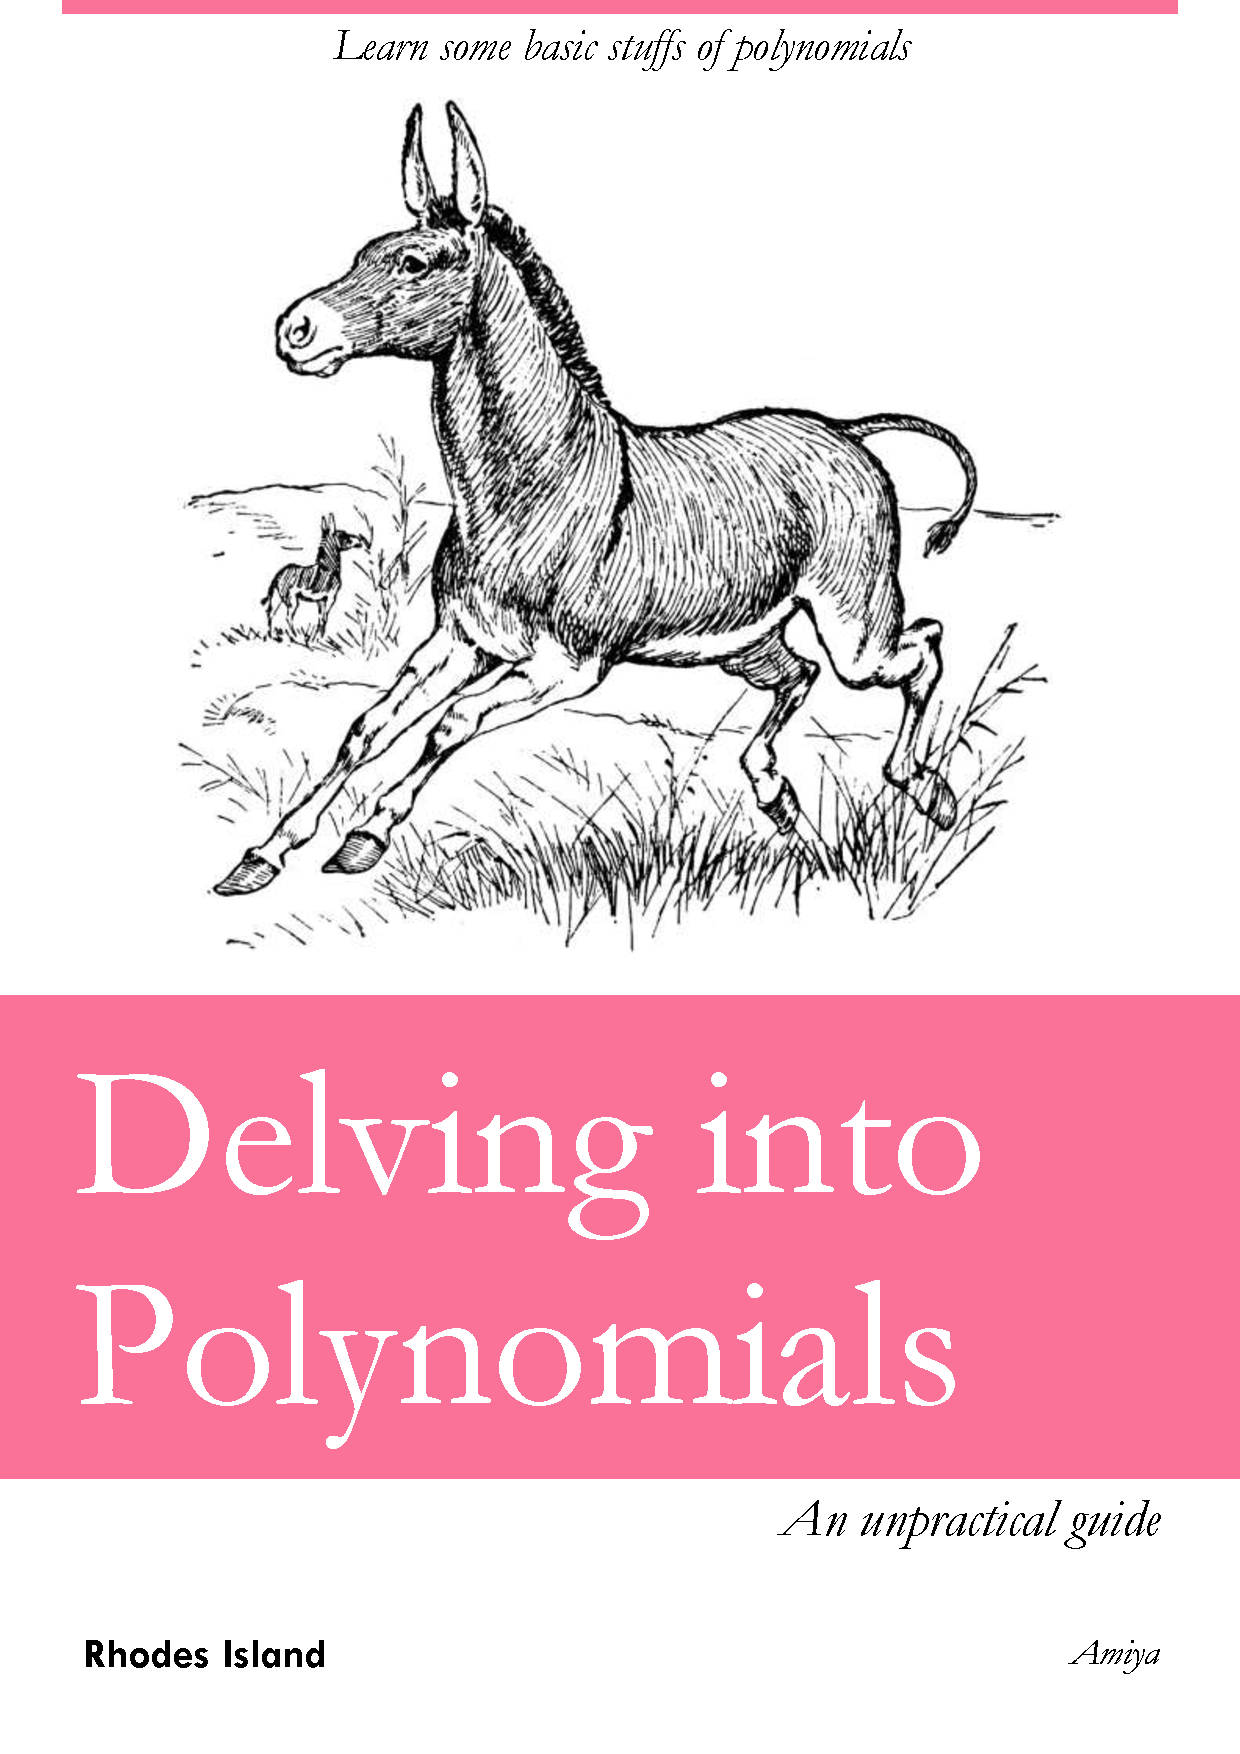
\includepdf{res/cover.pdf}
\ \
\clearpage

\title{}
\date{}
\author{}
\ctexset{today=old}
\pagestyle{plain}
\pagenumbering{roman}
\renewcommand{\contentsname}{Table of Contents}
\renewcommand{\abstractname}{Abstract}

\pagestyle{plain}
\thispagestyle{empty}
\tableofcontents

\newsection
\section*{Preface}
% Use the following line to add the unnumbered section to the table of contents
\addcontentsline{toc}{section}{Preface}

本文是瞎写的\period 我给本文的另一个名字是 ``Re: ゼロ から 始める ポリノミアル の イントロダクション''\period 不过想了想, 算了算了\period 龙鸣日语, 不好意思直接说出来\period

这是写给中学生看的\period

总是可以去这儿得到本文的最新版本:
\begin{align*}
    & \texttt{https://gitee.com/septsea/strange-book-zero} \\
    & \texttt{https://github.com/septsea/strange-book-zero}
\end{align*}

就先说到这里\period

\ \

\providecommand{\appendDate}{}
\renewcommand{\appendDate}[1]{\par \hfill {\itshape \sffamily #1}}

\begin{remark}
    总算写完 Prerequisites 了\period 我写这玩意儿花了好久好久啊\period 先发布再说吧\period
    \appendDate{June 3, 2021}
\end{remark}

\begin{remark}
    忘记介绍域是什么东西了\period 我真是笨蛋啊\period
    \appendDate{June 3, 2021}
\end{remark}


\newsection
\pagestyle{headings}
\setcounter{page}{1}
\pagenumbering{arabic}
\def\CC{\mathbb{C}}
\def\RR{\mathbb{R}}
\def\QQ{\mathbb{Q}}
\def\ZZ{\mathbb{Z}}
\def\NN{\mathbb{N}}
\def\FF{\mathbb{F}}
\def\ii{\mathrm{i}}
\def\myStar{\ding{72}}
\def\ellipsis{\dots}
\def\period{\text{。}}
\def\qedsymbol{\ding{44}}
\newcommand{ \term}[1]{(\textit{#1})}

\section*{Delving into Polynomials}
\addcontentsline{toc}{section}{Delving into Polynomials}
\markboth{Delving into Polynomials}{}

Out of boredom, I wrote the article.

    % This is used to occupy some space.
    {\vfill \itshape \sffamily \small
        \begin{center}
            \begin{tabular}{l}
                % /* cspell: disable-next-line */
                Gohan ni suru? Ofuro ni suru? Sore tomo\ellipsis \ wa ta shi? \\
                (Would you like dinner? Would you like a bath? Or\ellipsis \ would you like me?)
            \end{tabular}
        \end{center}}

\clearpage

\subsection*{Prerequisites}
\addcontentsline{toc}{subsection}{Prerequisites}
\markright{Prerequisites}

您将在本节熟悉一些记号与术语\period 不必细品\period 本节有很多定义\period 不要害怕: 就当是认识一下词语好了\period 本文主要讨论多项式, 所以并不会过多涉及到本节内容\period 说白了, 本节是工具节\period

\subsubsection*{Sets}

\begin{definition}
    集 \term{set} 是具有某种特定性质的对象汇集而成的一个整体, 其对象称为元 \term{element}\period
\end{definition}

\begin{definition}
    无元的集是空集 \term{empty set}\period
\end{definition}

\begin{remark}
    一般用小写字母表示元, 大写字母表示集\period
\end{remark}

\begin{definition}
    一般地, 若集 $A$ 由元 $a$, $b$, $c$, $\cdots$ 作成, 我们写
    \begin{align*}
        A = \{\, a,b,c,\cdots \,\} \period
    \end{align*}
    还有一种记号\period 设集 $A$ 是由具有某种性质 $p$ 的对象汇集而成, 则记
    \begin{align*}
        A = \{\, x \mid x \text{ possesses the property } p \,\} \period
    \end{align*}
\end{definition}

\begin{definition}
    若 $a$ 是集 $A$ 的元, 则写 $a \in A$ 或 $A \ni a$, 说 $a$ 属于 \term{to belong to} $A$ 或 $A$ 包含 \term{to contain} $a$\period 若 $a$ 不是集 $A$ 的元, 则写 $a \notin A$, 说 $a$ 不属于 $A$\period\myFN{有点尴尬, 我太菜了, 那个 ``不包含'' 符号打不出来\period}
\end{definition}

\begin{example}
    % /* cspell: disable-next-line */
    全体整数作成的集用 $\ZZ$ \term{Zahl}\myFN{A German word which means \textit{number}.} 表示\period 它可以写为
    \begin{align*}
        \ZZ = \{\, 0,1,-1,2,-2,\cdots,n,-n,\cdots \,\} \period
    \end{align*}
\end{example}

\begin{example}
    全体非负整数作成的集用 $\NN$ \term{natural} 表示\period 它可以写为
    \begin{align*}
        \NN = \{\, x \mid x \in \ZZ \text{ and } x \geq 0 \,\} \period
    \end{align*}
    为了方便, 也可以写为
    \begin{align*}
        \NN = \{\, x \in \ZZ \mid x \geq 0 \,\} \period
    \end{align*}
\end{example}

\begin{definition}
    若任取 $a \in A$, 都有 $a \in B$, 则写 $A \subset B$ 或 $B \supset A$, 说 $A$ 是 $B$ 的子集 \term{subset} 或 $B$ 是 $A$ 的超集 \term{superset}\period 假如有一个 $b \in B$ 不是 $A$ 的元, 可以用 ``真'' \term{proper} 形容之\period
\end{definition}

\begin{example}
    空集是任意集的子集\period 空集是任意不空的集的真子集\period
\end{example}

\begin{example}
    全体有理数作成的集用 $\QQ$ \term{quotient} 表示\period 因为整数是有理数, 所以 $\ZZ \subset \QQ$\period 因为有理数 $\frac12$ 不是整数, 我们说 $\ZZ$ 是 $\QQ$ 的真子集\period
\end{example}

\begin{definition}
    全体实数作成的集用 $\RR$ \term{real} 表示\period
\end{definition}

\begin{definition}
    全体复数作成的集用 $\CC$ \term{complex} 表示\period 不难看出,
    \begin{align*}
        \NN \subset \ZZ \subset \QQ \subset \RR \subset \CC \period
    \end{align*}
\end{definition}

\begin{definition}
    $\FF$ \term{field} 可表示 $\QQ$, $\RR$, $\CC$ 的任意一个\period 不难看出, $\FF$ 适合这几条:

    (i) $0 \in \FF$, $1 \in \FF$, $0 \neq 1$;

    (ii) 任取 $x,y \in \FF$ ($y \neq 0$), 必有 $x-y, \frac{x}{y} \in F$\period

    后面会见到稍详细的论述\period
\end{definition}

\begin{definition}
    设 $\mathbb{L}$ 是 $\CC$, $\RR$, $\QQ$, $\ZZ$, $\NN$, $\FF$ 的任意一个\period $\mathbb{L}^{\ast}$ 表示 $\mathbb{L}$ 去掉 $0$ 后得到的集\period 不难看出, $\mathbb{L}$ 是 $\mathbb{L}^{\ast}$ 的真超集\period
\end{definition}

\begin{definition}
    若集 $A$ 与 $B$ 包含的元完全一样, 则 $A$ 与 $B$ 是同一集\period 我们说 $A$ 等于 $B$, 写 $A = B$\period 显然
    \begin{align*}
        A = B \iff A \subset B \text{ and } B \subset A \period
    \end{align*}
\end{definition}

\begin{definition}
    集 $A$ 与 $B$ 的交 \term{intersection} 是集
    \begin{align*}
        A \cap B = \{\, x \mid x \in A \text{ and } x \in B \,\} \period
    \end{align*}
    也就是说, $A \cap B$ 恰由 $A$ 与 $B$ 的公共元作成\period

    集 $A$ 与 $B$ 的并 \term{union} 是集
    \begin{align*}
        A \cup B = \{\, x \mid x \in A \text{ or } x \in B \,\} \period
    \end{align*}
    也就是说, $A \cup B$ 恰包含 $A$ 与 $B$ 的全部元\period

    类似地, 可定义多个集的交与并\period
\end{definition}

\begin{definition}
    设 $A$, $B$ 是集\period 定义
    \begin{align*}
        A \times B = \{\, (a,b) \mid a \in A, \ b \in B  \,\} \period
    \end{align*}
    $A \times A$ 可简写为 $A^2$\period 类似地,
    \begin{align*}
        A \times B \times C = \{\, (a,b,c) \mid a \in A, \ b \in B, \ c \in C  \,\}, \quad A^3 = A \times A \times A \period
    \end{align*}
\end{definition}

\begin{example}
    设 $A = \{\, 1,2 \,\}$, $B = \{\, 3,4,5 \,\}$\period 则
    \begin{align*}
        A \times B = \{\, (1,3),(1,4),(1,5),(2,3),(2,4),(2,5) \,\}\period
    \end{align*}
    而
    \begin{align*}
        B \times A = \{\, (3,1),(3,2),(4,1),(4,2),(5,1),(5,2) \,\}\period
    \end{align*}
\end{example}

\begin{remark}
    一般地, $A \times B \neq B \times A$\period 假如 $A$, $B$ 各自有 $m$, $n$ 个元, 利用一点计数知识可以看出, $A \times B$ 有 $mn$ 个元\period
\end{remark}

\subsubsection*{Functions}

\begin{definition}
    假如通过一个法则 $f$, 使任取 $a \in A$, 都能得到唯一的 $b \in B$, 则说这个法则 $f$ 是集 $A$ 到集 $B$ 的一个函数 \term{function}\period 元 $b$ 是元 $a$ 在函数 $f$ 下的象 \term{image}\period 元 $a$ 是元 $b$ 在 $f$ 下的一个原象 \term{inverse image}\period 这个关系可以写为
    \begin{align*}
         & A \to B,  \tag*{$f$:}      \\
         & a \mapsto b = f(a) \period
    \end{align*}
    称 $A$ 是定义域 \term{domain}, $B$ 是陪域\myFN{不要混淆陪域与象集 (\textit{image}, \textit{range})\period $f$ 的象集是
        \begin{align*}
            \mathrm{Im} \, f = \{\, b \in B \mid b = f(a), \, a \in A \,\} \period
        \end{align*}
        这就是中学数学里的 ``值域''\period
        % /* cspell: disable-next-line */
    } \term{codomain}\period
\end{definition}

\begin{example}
    可以把 $\RR^2$ 看作平面上的点集\period 所以
    \begin{align*}
         & \RR^2 \to \RR,  \tag*{$f$:}  \\
         & (x,y) \mapsto \sqrt{x^2+y^2}
    \end{align*}
    是函数: 它表示点 $(x,y)$ 到点 $(0,0)$ 的距离\period
\end{example}

\begin{example}
    设
    \begin{align*}
         & A = \{\, \text{dinner}, \text{bath}, \text{me} \,\}, \quad B = \{\, 0,1 \,\} \period
    \end{align*}

    法则
    \begin{align*}
         & \text{dinner} \mapsto 0, \quad \text{bath} \mapsto 1 \tag*{$f_1$:}
    \end{align*}
    不是 $A$ 到 $B$ 的函数, 因为它没有为 $A$ 的元 $\text{me}$ 规定象\period 但是, 如果记 $A_1 = \{\, \text{dinner}, \text{bath} \,\}$, 这个 $f_1$ 可以是 $A_1$ 到 $B$ 的函数\period

    法则
    \begin{align*}
         & \text{dinner} \mapsto 0, \tag*{$f_2$:}          \\
         & \text{bath} \mapsto 1,                          \\
         & \text{me} \mapsto b \quad \text{where } b^2 = b
    \end{align*}
    不是 $A$ 到 $B$ 的函数, 因为它给 $A$ 的元 $\text{me}$ 规定的象不唯一\period

    法则
    \begin{align*}
         & \text{dinner} \mapsto 0, \quad
        \text{bath} \mapsto 1, \quad
        \text{me} \mapsto -1 \tag*{$f_3$:}
    \end{align*}
    不是 $A$ 到 $B$ 的函数, 因为它给 $A$ 的元 $\text{me}$ 规定的象不是 $B$ 的元\period 但是, 如果记 $B_1 = \{\, -1,0,1 \,\}$, 这个 $f_3$ 可以是 $A$ 到 $B_1$ 的函数\period
\end{example}

\begin{definition}
    设 $f_1$ 与 $f_2$ 都是 $A$ 到 $B$ 的函数\period 若任取 $a \in A$, 必有 $f_1 (a) = f_2 (a)$, 则说这二个函数相等, 写为 $f_1 = f_2$\period
\end{definition}

\begin{example}
    设 $A \subset \CC$, 且 $A$ 非空\period 定义二个 $A$ 到 $\CC$ 的函数: $f_1 (x) = x^2$, $f_2 (x) = |x|^2$\period 如果 $A = \RR$, 那么 $f_1 = f_2$\period 可是, 若 $A = \CC$, $f_1$ 与 $f_2$ 不相等\period
\end{example}

\begin{example}
    设 $A$ 是全体正实数作成的集\period 定义二个 $A$ 到 $\RR$ 的函数: $f_1 (x) = \frac16 \log_{2} {x^3}$, $f_2 (x) = \log_{4} {x}$\period 知道对数的读者可以看出, $f_1$ 与 $f_2$ 有着相同的对应法则, 故 $f_1 = f_2$\period 因为 $f_2$ 是对数函数 \term{logarithmic function}, 所以 $f_1$ 也是\period
\end{example}

\begin{remark}
    在上下文清楚的情况下, 可以单说函数的对应法则\period 比如, 中学数学课说 ``二次函数 $f(x) = x^2 + x - 1$'' 时, 定义域与陪域默认都是 $\RR$\period 中学的函数一般都是实数的子集到实数的子集的函数\period 所谓 ``自然定义域'' 是指 (在一定范围内) 一切使对应法则有意义的元构成的集\period 比如, 在中学, 我们说 $\frac{1}{x}$ 的自然定义域是 $\RR^{\ast}$, $\sqrt{x}$ 的自然定义域是一切非负实数\period 在研究复变函数时, 我们说 $\frac{1}{z}$ 的自然定义域是 $\CC^{\ast}$\period 如果不明确函数的定义域, 我们会根据上下文作出自然定义域作为它的定义域\period
\end{remark}

\begin{definition}
    $A$ 到 $A$ 的函数是 $A$ 的变换 \term{transform}\period 换句话说, 变换是定义域跟陪域一样的函数\period
\end{definition}

\subsubsection*{Binary Functions}

\begin{definition}
    $A^2$ 到 $A$ 的函数称为 $A$ 的二元运算 \term{binary functions}\period
\end{definition}

\begin{example}
    设 $f(x,y) = x-y$\period 这个 $f$ 是 $\ZZ$ 的二元运算; 但是, 它不是 $\NN$ 的二元运算\period
\end{example}

\begin{remark}
    设 $\circ$ 是 $A$ 的二元运算\period 代替 $\circ (x,y)$, 我们写 $x \circ y$\period 一般地, 若表示这个二元运算的符号不是字母, 我们就把这个符号写在二个元的中间\period
\end{remark}

\begin{definition}
    设 $T(A)$ 是全部 $A$ 的变换作成的集\period 设 $f,g$ 是 $A$ 的变换\period 任取 $a \in A$, 当然有 $b = f(a) \in A$\period 所以, $g(b) = g(f(a))$ 也是 $A$ 的元\period 当然, 这个 $g(f(a))$ 也是唯一确定的\period 这样, 我们说, $f$ 与 $g$ 的复合 \term{composition} $g \circ f$ 是
    \begin{align*}
         & A \to A, \tag*{$g \circ f \colon$} \\
         & a \mapsto g(f(a)) \period
    \end{align*}
    所以, 复合是 $T(A)$ 的二元运算:
    \begin{align*}
         & T(A) \times T(A) \to T(A), \tag*{$\circ \colon$} \\
         & (g,f) \mapsto g \circ f \period
    \end{align*}
\end{definition}

\begin{remark}
    设 $A$ 有有限多个元\period 此时, 可排出 $A$ 的元:
    \begin{align*}
        A = \{\, a_1, a_2, \cdots, a_n \,\} \period
    \end{align*}
    设 $f$ 是 $A^2$ 到 $B$ 的函数\period 则任给整数 $i,j$, $1 \leq i,j \leq n$, 记
    \begin{align*}
        f(a_i, a_j) = b_{i,j} \in B \period
    \end{align*}
    可以用这样的表描述此函数:
    \begin{align*}
        \arraycolsep=0.25cm
        \begin{array}{c|cccc}
            \      & a_1     & a_2     & \cdots & a_n     \\ \hline
            a_1    & b_{1,1} & b_{1,2} & \cdots & b_{1,n} \\
            a_2    & b_{2,1} & b_{2,2} & \cdots & b_{2,n} \\
            \vdots & \vdots  & \vdots  & \ddots & \vdots  \\
            a_n    & b_{n,1} & b_{n,2} & \cdots & b_{n,n} \\
        \end{array}
    \end{align*}
    有的时候, 为了强调函数名, 可在左上角书其名:
    \begin{align*}
        \arraycolsep=0.25cm
        \begin{array}{c|cccc}
            f      & a_1     & a_2     & \cdots & a_n     \\ \hline
            a_1    & b_{1,1} & b_{1,2} & \cdots & b_{1,n} \\
            a_2    & b_{2,1} & b_{2,2} & \cdots & b_{2,n} \\
            \vdots & \vdots  & \vdots  & \ddots & \vdots  \\
            a_n    & b_{n,1} & b_{n,2} & \cdots & b_{n,n} \\
        \end{array}
    \end{align*}
    这种表示函数的方式是方便的\period 如果这些 $b_{i,j}$ 都是 $A$ 的元, 就说这张表是 $A$ 的运算表\period
\end{remark}

\begin{example}
    设 $T = \{\, 0,1,-1 \,\}$, $\circ (x,y) = xy$\period 不难看出, $\circ$ 确实是 $T$ 的二元运算\period 它的运算表如下:
    \begin{align*}
        \arraycolsep=0.25cm
        \begin{array}{c|ccc}
            \  & 0 & 1  & -1 \\ \hline
            0  & 0 & 0  & 0  \\
            1  & 0 & 1  & -1 \\
            -1 & 0 & -1 & 1  \\
        \end{array}
    \end{align*}
\end{example}

\begin{example}
    设 $\FF_{\mathrm{nu}}$ 是将 $\FF$ 去掉 $0$, $1$ 后得到的集\myFN{这个 $\FF_{\mathrm{nu}}$ 只是临时记号: $\mathrm{nu}$ 表示 \textit{nil}, \textit{unity}\period}\period 看下列 $6$ 个法则:
    \begin{align*}
         & x \mapsto x; \tag*{$f_0 \colon$}                   \\
         & x \mapsto 1-x; \tag*{$f_1 \colon$}                 \\
         & x \mapsto \frac{1}{x}; \tag*{$f_2 \colon$}         \\
         & x \mapsto 1-\frac{1}{1-x}; \tag*{$f_3 \colon$}     \\
         & x \mapsto 1-\frac{1}{x}; \tag*{$f_4 \colon$}       \\
         & x \mapsto \frac{1}{1-x}\period \tag*{$f_5 \colon$}
    \end{align*}
    记 $S_6 = \{\, f_0,f_1,f_2,f_3,f_4,f_5 \,\}$\period 可以验证, $S_6 \subset T(\FF_{\mathrm{nu}})$\period

    进一步地, $36$ 次复合告诉我们, 任取 $f,g \in S_6$, 必有 $g \circ f \in S_6$\period 可以验证, 这是 $S_6$ 的 (复合) 运算表:
    \begin{align*}
        \arraycolsep=0.25cm
        \begin{array}{c|cccccc}
            \     & f_{0} & f_{1} & f_{2} & f_{3} & f_{4} & f_{5} \\ \hline
            f_{0} & f_{0} & f_{1} & f_{2} & f_{3} & f_{4} & f_{5} \\
            f_{1} & f_{1} & f_{0} & f_{4} & f_{5} & f_{2} & f_{3} \\
            f_{2} & f_{2} & f_{5} & f_{0} & f_{4} & f_{3} & f_{1} \\
            f_{3} & f_{3} & f_{4} & f_{5} & f_{0} & f_{1} & f_{2} \\
            f_{4} & f_{4} & f_{3} & f_{1} & f_{2} & f_{5} & f_{0} \\
            f_{5} & f_{5} & f_{2} & f_{3} & f_{1} & f_{0} & f_{4} \\
        \end{array}
    \end{align*}

    我们在本节会经常用 $S_6$ 举例\period
\end{example}

\begin{definition}
    设 $\circ$ 是 $A$ 的二元运算\period 若任取 $x,y,z \in A$, 必有
    \begin{align*}
        (x \circ y) \circ z = x \circ (y \circ z),
    \end{align*}
    则说 $f$ 适合结合律 \term{associativity}\period 此时, $(x \circ y) \circ z$ 或 $x \circ (y \circ z)$ 可简写为 $x \circ y \circ z$\period
\end{definition}

\begin{example}
    $\ZZ$ 的加法当然适合结合律\period 可是, 它的减法不适合结合律\period
\end{example}

\begin{remark}
    变换的复合适合结合律\period 确切地, 设 $f,g,h$ 都是 $A$ 的变换\period 任取 $a \in A$, 则
    \begin{align*}
         & (h \circ (g \circ f))(a) = h((g \circ f)(a)) = h(g(f(a))),        \\
         & ((h \circ g) \circ f)(a) = (h \circ g)(f(a)) = h(g(f(a))) \period
    \end{align*}
    也就是说,
    \begin{align*}
        h \circ (g \circ f) = (h \circ g) \circ f \period
    \end{align*}
\end{remark}

\begin{example}
    $S_6$ 的复合当然适合结合律\period
\end{example}

\begin{definition}
    设 $\circ$ 是 $A$ 的二元运算\period 若任取 $x,y \in A$, 必有
    \begin{align*}
        x \circ y = y \circ x,
    \end{align*}
    则说 $\circ$ 适合交换律 \term{commutativity}\period
\end{definition}

\begin{example}
    $\FF^{\ast}$ 的乘法当然适合交换律\period 可是, 它的除法不适合交换律\period
\end{example}

\begin{example}
    $S_6$ 的复合不适合交换律, 因为 $f_1 \circ f_2 = f_4$, 而 $f_2 \circ f_1 = f_5$, 二者不相等\period
\end{example}

\begin{remark}
    在本文里, $\cdot$ 运算的优先级高于 $+$ 运算\period 所以, $a \cdot b + c$ 的意思就是
    \begin{align*}
        (a \cdot b) + c,
    \end{align*}
    而不是
    \begin{align*}
        a \cdot (b + c)\period
    \end{align*}
\end{remark}

\begin{definition}
    设 $+$, $\cdot$ 是 $A$ 的二个二元运算\period 若任取 $x,y,z \in A$, 必有
    \begin{align*}
         & x \cdot (y + z) = x \cdot y + x \cdot z, \tag*{(LD)}
    \end{align*}
    则说 $+$ 与 $\cdot$ 适合左 ($\cdot$) 分配律\myFN{在不引起歧义时, 括号里的内容可省略\period 或者这么说: 当我们说 $+$, $\cdot$ 适合分配律时, 我们不会理解为 $x + (y \cdot z) = (x + y) \cdot (x + z)$\period 但有意思的是, 如果把 $+$ 理解为并, $\cdot$ 理解为交, $x$, $y$, $z$ 理解为集, 那这个式子是对的\period 当然, $x \cdot (y + z) = x \cdot y + x \cdot z$ 也是对的\period} \term{left distributivity}\period 类似地, 若
    \begin{align*}
         & (y + z) \cdot x = y \cdot x + z \cdot x, \tag*{(RD)}
    \end{align*}
    则说 $+$ 与 $\cdot$ 适合右 ($\cdot$) 分配律 \term{right distributivity}\period 说既适合 LD 也适合 RD 的 $+$ 与 $\cdot$ 适合 ($\cdot$) 分配律 \term{distributivity}\period 显然, 若 $\cdot$ 适合交换律, 则 LD 与 RD 等价\period
\end{definition}

\begin{example}
    $\FF$ 的加法与乘法适合分配律\period 当然, 减法与乘法也适合分配律:
    \begin{align*}
        x(y-z) = xy - xz = yx - zx = (y-z)x \period
    \end{align*}
    甚至, 在正实数里, 加法与除法适合右分配律:
    \begin{align*}
        \frac{y+z}{x} = \frac{y}{x} + \frac{z}{x} \period
    \end{align*}
\end{example}

\begin{definition}
    设 $\circ$ 是 $A$ 的二元运算\period 若任取 $x,y,z \in A$, 必有
    \begin{align*}
         & x \circ y = x \circ z \implies y = z, \tag*{(LC)}
    \end{align*}
    则说 $\circ$ 适合左消去律 \term{left cancellation property}\period 类似地, 若
    \begin{align*}
         & x \circ z = y \circ z \implies x = y, \tag*{(RC)}
    \end{align*}
    则说 $\circ$ 适合右消去律 \term{right cancellation property}\period 说既适合 LC 也适合 RC 的 $\circ$ 适合消去律 \term{cancellation property}\period 显然, 若 $\circ$ 适合交换律, 则 LC 与 RC 等价\period
\end{definition}

\begin{example}
    显然, $\NN$ 的乘法不适合消去律, 但 $\NN^{\ast}$ 的乘法适合消去律\myFN{后面提到整环时, 我们会稍微修改一下消去律的描述\period}\period
\end{example}

\begin{example}
    考虑 $x \circ y = x^3 + y^2$\period 若把 $\circ$ 视为 $\NN$ 的二元运算, 那么它适合消去律\period 若把 $\circ$ 视为 $\QQ$ 的二元运算, 那么它适合右消去律\period 若把 $\circ$ 视为 $\CC$ 的二元运算, 那么它不适合任意一个消去律\period
\end{example}

\begin{example}
    一般地, 当 $A$ 至少有二个元时, $\circ$ (在 $T(A)$ 里) 不适合消去律\period 设 $a,b \in A$, $a \neq b$\period 考虑下面 $4$ 个变换:
    \begin{align*}
         & a \mapsto a, \quad b \mapsto b, \quad x \mapsto x \text{ where $x \neq a,b$}; \tag*{$g_0 \colon$}       \\
         & a \mapsto a, \quad b \mapsto a, \quad x \mapsto x \text{ where $x \neq a,b$}; \tag*{$g_1 \colon$}       \\
         & a \mapsto b, \quad b \mapsto b, \quad x \mapsto x \text{ where $x \neq a,b$}; \tag*{$g_2 \colon$}       \\
         & a \mapsto b, \quad b \mapsto a, \quad x \mapsto x \text{ where $x \neq a,b$}\period \tag*{$g_3 \colon$}
    \end{align*}
    可以验证,
    \begin{align*}
        g_3 \circ g_1 = g_2 \circ g_1 = g_2 \circ g_3 = g_2 \period
    \end{align*}
    由此可以看出, $\circ$ 不适合任意一个消去律\period
\end{example}

\begin{example}
    我们看 $\circ$ 在 $S_6$ 里是否适合消去律\period 取 $f,g,h \in S_6$\period 由表易知, 当 $g \neq h$ 时, $f \circ g \neq f \circ h$ (横着看运算表), 且 $g \circ f \neq h \circ f$ (竖着看运算表)\period 这说明, $\circ$ 在 $T(\FF_{\mathrm{nu}})$ 的子集 $S_6$ 里适合消去律\period
\end{example}

\begin{definition}
    设 $\circ$ 是 $A$ 的二元运算\period 若存在 $e \in A$, 使若任取 $x \in A$, 必有
    \begin{align*}
        e \circ x = x \circ e = x,
    \end{align*}
    则说 $e$ 是 $A$ 的 (关于运算 $\circ$ 的) 幺元 \term{identity}\period 如果 $e^{\prime}$ 也是幺元, 则
    \begin{align*}
        e = e \circ e^{\prime} = e^{\prime} \period
    \end{align*}
\end{definition}

\begin{example}
    $\FF$ 的加法的幺元是 $0$, 且其乘法的幺元是 $1$\period
\end{example}

\begin{example}
    不难看出, 这个变换是 $T(A)$ 的幺元:
    \begin{align*}
         & A \to A,  \tag*{$\iota$:} \\
         & a \mapsto a \period
    \end{align*}
    它也有个一般点的名字: 恒等变换 \term{identity transform}\period

    在 $S_6$ 里, $f_0$ 就是这里的 $\iota$\period
\end{example}

\begin{definition}
    设 $\circ$ 是 $A$ 的二元运算\period 设 $x \in A$ 若存在 $y \in A$, 使
    \begin{align*}
        y \circ x = x \circ y = e,
    \end{align*}
    则说 $y$ 是 $x$ 的 (关于运算 $\circ$ 的) 逆元 \term{inverse}\period
\end{definition}

\begin{example}
    $\FF$ 的每个元都有加法逆元, 即其相反数\period
\end{example}

\begin{remark}
    设 $\circ$ 适合结合律\period 如果 $y, y^{\prime}$ 都是 $x$ 的逆元, 则
    \begin{align*}
        y = y \circ e = y \circ (x \circ y^{\prime}) = (y \circ x) \circ y^{\prime} = e \circ y^{\prime} = y^{\prime} \period
    \end{align*}
    此时, 一般用 $x^{-1}$ 表示 $x$ 的逆元\period 因为
    \begin{align*}
        x^{-1} \circ x = x \circ x^{-1} = e,
    \end{align*}
    由上可知, $x^{-1}$ 也有逆元, 且 $(x^{-1})^{-1} = x$\period
\end{remark}

\begin{example}
    一般地, 当 $A$ 至少有二个元时, $T(A)$ 既有有逆元的变换, 也有无逆元的变换\period 还是看前面的 $g_0$, $g_1$, $g_2$, $g_3$\period 首先, $g_0$ 是幺元 $\iota$\period 不难看出, $g_0$ 与 $g_3$ 都有逆元:
    \begin{align*}
         & g_0 \circ g_0 = g_3 \circ g_3 = g_0 \period
    \end{align*}
    不过, $g_1$ 不可能有逆元\period 假设 $g_1$ 有逆元 $h$, 则应有
    \begin{align*}
        (h \circ g_1)(a) = \iota(a) = a, \quad (h \circ g_1)(b) = \iota(b) = b \period
    \end{align*}
    可是, $g_1(a) = g_1(b) = a$, 故 $(h \circ g_1)(a) = (h \circ g_1)(b) = h(a)$, 它不能既等于 $a$ 也等于 $b$, 矛盾!
\end{example}

\begin{example}
    再看 $S_6$\period 由表可看出, $f_0$, $f_1$, $f_2$, $f_3$, $f_4$, $f_5$ 的逆元分别是 $f_0$, $f_1$, $f_2$, $f_3$, $f_5$, $f_4$\period
\end{example}

\begin{remark}
    设 $\circ$ 适合结合律\period 如果 $x,y$ 都有逆元, 那么 $x \circ y$ 也有逆元, 且
    \begin{align*}
        (x \circ y)^{-1} = y^{-1} \circ x^{-1} \period
    \end{align*}
    为了说明这一点, 只要按定义验证即可:
    \begin{align*}
         & (y^{-1} \circ x^{-1}) \circ (x \circ y) = y^{-1} \circ (x^{-1} \circ x) \circ y = y^{-1} \circ e \circ y = y^{-1} \circ y = e,        \\
         & (x \circ y) \circ (y^{-1} \circ x^{-1}) = x \circ (y \circ y^{-1}) \circ x^{-1} = x \circ e \circ x^{-1} = x \circ x^{-1} = e \period
    \end{align*}
    这个规则往往称为袜靴规则 \term{socks and shoes rule}: 设 $y$ 是穿袜, $x$ 是穿靴, $x \circ y$ 表示动作的复合: 先穿袜后穿靴\period 那么这个规则告诉我们, $x \circ y$ 的逆元就是先脱靴再脱袜\period
\end{remark}

\begin{remark}
    由此可见, 结合律是一条很重要的规则\period 我们算 $63 \cdot 8 \cdot 125$ 时也会想着先算 $8 \cdot 125$\period
\end{remark}

\subsubsection*{Semi-groups and Groups}

\begin{definition}
    设 $S$ 是非空集\period 设 $\circ$ 是 $S$ 的二元运算\period 若 $\circ$ 适合结合律, 则称 $S$ (关于 $\circ$) 是半群 \term{semi-group}\period
\end{definition}

\begin{example}
    $\NN$ 关于加法 (或乘法) 作成半群\period
\end{example}

\begin{example}
    $T(A)$ 关于 $\circ$ 作成半群\period
\end{example}

\begin{remark}
    事实上, 这里要求 $S$ 非空是有必要的\period

    首先, 空集没什么意思\period 其次, 前面所述的结合律、交换律、分配律等自动成立, 这是因为对形如 ``若 $p$, 则 $q$'' 的命题 \term{proposition} 而言, $p$ 为假推出整个命题为真\period 这是相当 ``危险'' 的!
\end{remark}

\begin{definition}
    设 $m$ 是正整数\period 设 $x$ 是半群 $S$ 的元\period 令
    \begin{align*}
        x^{1} = x, \quad x^{m} = x \circ x^{m-1} \period
    \end{align*}
    $x^{m}$ 称为 $x$ 的 $m$ 次幂\period 不难看出, 当 $m,n$ 都是正整数时,
    \begin{align*}
        x^{m+n} = x^m \circ x^n, \quad (x^m)^n = x^{mn} \period
    \end{align*}
    假如 $S$ 有二个元 $x$, $y$ 适合 $x \circ y = y \circ x$, 那么还有
    \begin{align*}
        (x \circ y)^m = x^m \circ y^m \period
    \end{align*}
\end{definition}

\begin{example}
    还是看熟悉的 $\NN$\period 对于乘法而言, 这里的幂就是普通的幂——一个数自乘多次的结果\period 对于加法而言, 这里的幂相当于乘法——一个数自加多次的结果\period
\end{example}

\begin{definition}
    设 $G$ 关于 $\circ$ 是半群\period 若 $G$ 的关于 $\circ$ 的幺元存在, 且 $G$ 的任意元都有关于 $\circ$ 的逆元, 则 $G$ 是群 \term{group}\period
\end{definition}

\begin{example}
    $\NN$ 关于加法 (或乘法) 不能作成群\period $\ZZ$ 关于加法作成群, 但关于乘法不能作成群\period $\FF$ 关于乘法不能作成群, 但 $\FF^{\ast}$ 关于乘法作成群\period 不过, $\FF^{\ast}$ 关于加法不能作成群\period
\end{example}

\begin{example}
    $T(A)$ 一般不是群\period 不过, $S_6$ 是群\period
\end{example}

\begin{remark}
    群有唯一的幺元\period 群的每个元都有唯一的逆元\period
\end{remark}

\begin{remark}
    设 $G$ 关于 $\circ$ 是群\period 我们说, $\circ$ 适合消去律\period

    假如 $x \circ y = x \circ z$\period 二侧左边乘 $x$ 的逆元 $x^{-1}$, 就有
    \begin{align*}
        x^{-1} \circ (x \circ y) = x^{-1} \circ (x \circ y) \period
    \end{align*}
    由于 $\circ$ 适合结合律,
    \begin{align*}
        (x^{-1} \circ x) \circ y = (x^{-1} \circ x) \circ y \period
    \end{align*}
    也就是
    \begin{align*}
        e \circ y = e \circ z \period
    \end{align*}
    这样, $y = z$\period 类似地, 用同样的方法可以知道, 右消去律也对\period
\end{remark}

\begin{definition}
    已经知道, 群的每个元 $x$ 都有逆元 $x^{-1}$\period 由此, 当 $m$ 是正整数时, 定义 $x^{-m} = (x^{-1})^m$\period 再定义 $x^0 = e$\period 利用半群的结果, 可以看出, 当 $m,n$ 都是整数时,
    \begin{align*}
        x^{m+n} = x^m \circ x^n, \quad (x^m)^n = x^{mn} \period
    \end{align*}
    假如 $G$ 有二个元 $x$, $y$ 适合 $x \circ y = y \circ x$, 那么还有
    \begin{align*}
        (x \circ y)^m = x^m \circ y^m \period
    \end{align*}
\end{definition}

\begin{example}
    对于 $\FF^{\ast}$ 的乘法而言, 这里的任意整数幂跟普通的整数幂没有任何区别\period 我们学习数的负整数幂的时候, 也是借助倒数定义的\period
\end{example}

\subsubsection*{Subgroups}

\begin{definition}
    设 $G$ 关于 $\circ$ 是群\period 设 $H \subset G$, $H$ 非空\period 若 $H$ 关于 $\circ$ 也作成群, 则 $H$ 是 $G$ 的子群 \term{subgroup}\period
\end{definition}

\begin{example}
    对加法来说, $\ZZ$ 是 $\FF$ 的子群\period 对乘法来说, $\ZZ^{\ast}$ 不是 $\FF^{\ast}$ 的子群\period
\end{example}

\begin{remark}
    设 $H \subset G$, $H$ 非空\period $H$ 是 $G$ 的子群的一个必要与充分条件是: 任取 $x,y \in H$, 必有 $x \circ y^{-1} \in H$\period

    怎么说明这一点呢? 先看充分性\period 任取 $x \in H$, 则 $e = x \circ x^{-1} \in H$\period 任取 $y \in H$, 则 $y^{-1} = e \circ y^{-1} \in H$\period 所以
    \begin{align*}
        x \circ y = x \circ (y^{-1})^{-1} \in H \period
    \end{align*}
    $\circ$ 在 $G$ 适合结合律, $H \subset G$, 所以 $\circ$ 作为 $H$ 的二元运算也适合结合律\period 至此, $H$ 是半群\period

    前面已经说明, $e \in H$, 所以 $H$ 的关于 $\circ$ 的幺元存在\period 进一步地, $x \in H$ 在 $G$ 里的逆元也是 $H$ 的元, 所以 $H$ 的任意元都有关于 $\circ$ 的逆元\period 这样, $H$ 是群\period 顺便一提, 我们刚才也说明了, $G$ 的幺元也是 $H$ 的幺元, 且 $H$ 的元在 $G$ 里的逆元也是在 $H$ 里的逆元\period

    再看必要性\period 假设 $H$ 是一个群\period 任取 $x,y \in H$, 我们要说明 $x \circ y^{-1} \in H$\period 看上去有点显然呀! $H$ 是群, 所以 $y$ 有逆元 $y^{-1}$, 又因为 $\circ$ 是 $H$ 的二元运算, $x \circ y^{-1} \in H$\period 不过要注意一个细节\period 我们说明充分性时, $y^{-1}$ 被认为是 $y$ 在 $G$ 里的逆元; 可是, 刚才的论证里 $y^{-1}$ 实则是 $y$ 在 $H$ 里的逆元\period 大问题! 怎么解决呢? 如果我们说明 $y$ 在 $H$ 里的逆元也是 $y$ 在 $G$ 里的逆元, 那这个漏洞就被修复了\period

    我们知道, $H$ 有幺元 $e_H$, 所以 $e_H \circ e_H = e_H$\period $e_H$ 是 $G$ 的元, 所以 $e_H$ 在 $G$ 里有逆元 $(e_H)^{-1}$\period 这样,
    \begin{align*}
        e_H
        = \  & e \circ e_H                      \\
        = \  & ((e_H)^{-1} \circ e_H) \circ e_H \\
        = \  & (e_H)^{-1} \circ (e_H \circ e_H) \\
        = \  & (e_H)^{-1} \circ e_H             \\
        = \  & e \period
    \end{align*}
    取 $y \in H$\period $y$ 在 $H$ 里有逆元 $z$, 即
    \begin{align*}
        z \circ y = y \circ z = e_H = e\period
    \end{align*}
    $y$, $z$ 都是 $G$ 的元\period 这样, 根据逆元的唯一性, $z$ 自然是 $y$ 在 $G$ 里的逆元\period
\end{remark}

\subsubsection*{Additive Groups}

\begin{definition}
    若 $G$ 关于名为 $+$ 的二元运算作成群, 幺元 $e$ 读作 ``零元'' 写作 $0$, $x \in G$ 的逆元 $x^{-1}$ 读作 ``$x$ 的相反元'' 写作 $-x$, 且 $+$ 适合交换律, 则说 $G$ 是加群 \term{additive group}\period 相应地, ``元的幂'' 也应该改为 ``元的倍'': $x^m$ 写为 $mx$\period 用加法的语言改写前面的幂的规则, 就得到了倍的规则: 对任意 $x,y \in G$, $m,n \in \ZZ$, 有
    \begin{align*}
         & (m+n)x = mx + nx,       \\
         & m(nx) = (mn)x,          \\
         & m(x+y) = mx + my\period
    \end{align*}
    顺便一提, 在这种记号下, $x-y$ 是 $x+(-y)$ 的简写\period 并且
    \begin{align*}
        x + y = x + z \implies y = z\period
    \end{align*}
    由于这里的加法适合交换律, 直接换位就是右消去律\period 前面说, 若运算适合结合律, 则 $x$ 的逆元的逆元还是 $x$\period 这句话用加法的语言写, 就是
    \begin{align*}
        -(-x) = x\period
    \end{align*}
    前面的 ``袜靴规则'' 就是
    \begin{align*}
        -(x+y) = (-y) + (-x) = (-x) + (-y) = -x-y\period
    \end{align*}
    这就是熟悉的去括号法则\period 这里体现了交换律的作用\period
\end{definition}

\begin{remark}
    初见此定义可能会觉得有些混乱: 怎么 ``倒数'' 又变为 ``相反数'' 了? 其实这都是借鉴已有写法\period 前面, $\circ$ 虽然不是 $\cdot$, 但这个形状暗示着乘法, 因此有 $x^{-1}$ 这样的记号; 现在, 运算的名字是 $+$, 自然要根据形状作出相应的改变\period 其实, 这里 ``名为 $+$'' ``零元'' ``相反元'' 都不是本质——换句话说, 还是可以用老记号\period 不过, 我们主要接触至少与二种运算相关联的结构——整环与域, 所以用二套记号、名字是有必要的\period
\end{remark}

\begin{remark}
    前面的 $x^0 = e$ 在加群里变为 $0x = 0$\period 看上去 ``很普通'', 不过左边的 $0$ 是整数, 右边的 $0$ 是加群的零元, 二者一般不一样!
\end{remark}

\begin{example}
    显而易见, $\ZZ$, $\FF$ 都是加群\period
\end{example}

\begin{example}
    $S_6$ 不是加群, 因为它的二元运算不适合交换律\period
\end{example}

\begin{remark}
    类似地, 可以定义子加群 \term{sub-additive group}\period 这里, 就直接用等价刻画来描述它: ``$G$ 的非空子集 $H$ 是加群 $G$ 的子加群的一个必要与充分条件是: 任取 $x,y \in H$, 必有 $x-y \in H$\period ''
\end{remark}

\subsubsection*{Sums}

\begin{definition}
    设 $f$ 是 $\ZZ$ 的非空子集 $S$ 到加群 $G$ 的函数\period 设 $p$, $q$ 是二个整数\period 如果 $p \leq q$, 则记
    \begin{align*}
        \sum_{j = p}^{q} f(j) = f(p) + f(p + 1) + \cdots + f(q)\period
    \end{align*}
    也就是说, $\sum_{j = p}^{q} f(j)$ 就是 $q - (p - 1)$ 个元的和的一种简洁的表示法\period 如果 $p > q$, 约定 $\sum_{j = p}^{q} f(j) = 0$\period
\end{definition}

\begin{example}
    我们已经知道, $n \geq 0$ 时
    \begin{align*}
        0 + 1 + \cdots + (n-1) = \frac{n(n-1)}{2}\period
    \end{align*}
    用 $\sum$ 写出来, 就是
    \begin{align*}
        \sum_{k=0}^{n-1} k = \frac{n(n-1)}{2}\period
    \end{align*}
    这里的 $k$ 是所谓的 ``dummy variable''\period 所以,
    \begin{align*}
        \sum_{j=0}^{n-1} j = \sum_{k=0}^{n-1} k = \sum_{\ell=0}^{n-1} \ell = \frac{n(n-1)}{2}\period
    \end{align*}
\end{example}

\begin{example}
    $f$ 可以是常函数:
    \begin{align*}
        \sum_{t=p}^{q} 1 = \begin{cases}
            q - p + 1, & \quad q \geq p;     \\
            0,         & \quad q < p \period
        \end{cases}
    \end{align*}
\end{example}

\begin{example}
    设 $f$ 与 $g$ 是 $\ZZ$ 的非空子集 $S$ 到加群 $G$ 的函数\period 因为加群的加法适合结合律与交换律, 所以
    \begin{align*}
        \sum_{j=p}^{q} (f(j) + g(j)) = \sum_{j=p}^{q} f(j) + \sum_{j=p}^{q} g(j) \period
    \end{align*}
\end{example}

\begin{remark}
    设 $f(i,j)$ 是 $\ZZ^2$ 的非空子集到加群 $G$ 的函数\period 记
    \begin{align*}
        S_C = \sum_{j=p}^{q} \sum_{i=m}^{n} f(i,j), \quad S_R = \sum_{i=m}^{n} \sum_{j=p}^{q} f(i,j),
    \end{align*}
    其中 $q \geq p$, $n \geq m$\period $\sum_{i=m}^{n} f(i,j)$ 是何物? 暂时视 $i$ 之外的变元为常元, 则
    \begin{align*}
        \sum_{i=m}^{n} f(i,j) = f(m,j) + f(m+1,j) + \cdots + f(n,j) \period
    \end{align*}
    $\sum_{j=p}^{q} \sum_{i=m}^{n} f(i,j)$ 是 $\sum_{j=p}^{q} \left( \sum_{i=m}^{n} f(i,j) \right)$ 的简写:
    \begin{align*}
        \sum_{j=p}^{q} \sum_{i=m}^{n} f(i,j) = \sum_{i=m}^{n} f(i,p) + \sum_{i=m}^{n} f(i,p+1) + \cdots + \sum_{i=m}^{n} f(i,q) \period
    \end{align*}
    $\sum_{i=m}^{n} \sum_{j=p}^{q} f(i,j)$ 有着类似的解释\period 我们说, $S_C$ 一定与 $S_R$ 相等\period

    记
    \begin{align*}
        C_j = \sum_{i=m}^{n} f(i,j), \quad R_i = \sum_{j=p}^{q} f(i,j) \period
    \end{align*}
    考虑下面的表:
    \begin{align*}
        \begin{array}{cccc|c}
            f(m,p)   & f(m,p+1)   & \cdots & f(m,q)   & R_{m}   \\
            f(m+1,p) & f(m+1,p+1) & \cdots & f(m+1,q) & R_{m+1} \\
            \vdots   & \vdots     & \ddots & \vdots   & \vdots  \\
            f(n,p)   & f(n,p+1)   & \cdots & f(n,q)   & R_{n}   \\ \hline
            C_{p}    & C_{p+1}    & \cdots & C_{q}    & \
        \end{array}
    \end{align*}
    由此, 不难看出, $S_C$ 与 $S_R$ 只是用不同的方法将 $(n-m+1)(q-p+1)$ 个元相加罢了\period
\end{remark}

\begin{remark}
    上面的例其实就是一个特殊情形 ($n - m = 1$)\period
\end{remark}

\subsubsection*{Rings}

\begin{definition}
    设 $R$ 是加群\period 设 $\cdot$ (读作 ``乘法'') 也是 $R$ 的二元运算\period 假设

    (i) $\cdot$ 适合结合律;

    (ii) $+$ 与 $\cdot$ 适合 $\cdot$ 分配律\period

    我们说 $R$ (关于 $+$ 与 $\cdot$) 是环 \term{ring}\period
\end{definition}

\begin{remark}
    在不引起歧义的情况下, 可省去 $\cdot$ \, \period 例如, $a \cdot b$ 可写为 $ab$\period
\end{remark}

\begin{example}
    $\ZZ$, $\FF$ (关于普通加法与乘法) 都是环\period
\end{example}

\begin{example}
    全体偶数作成的集也是环\period 一般地, 设 $k$ 是整数, 则全体 $k$ 的倍作成的集是环\period
\end{example}

\begin{example}
    这里举一个 ``平凡的'' \term{trivial} 例\period $N$ 只有一个元 $0$\period 可以验证, $N$ 关于普通加法与乘法作成群\period 这也是 ``最小的环''\period 在上个例里, 取 $k=0$ 就是 $N$\period
\end{example}

\begin{example}
    这里举一个 ``不平凡的'' \term{nontrivial} 例\period 设 $R = \{\, 0,a,b,c \,\}$\period 加法和乘法由以下二个表给定:
    \begin{align*}
        \arraycolsep=0.25cm
        \begin{array}{c|cccc}
            + & 0 & a & b & c \\ \hline
            0 & 0 & a & b & c \\
            a & a & 0 & c & b \\
            b & b & c & 0 & a \\
            c & c & b & a & 0 \\
        \end{array}
        \qquad \qquad
        \begin{array}{c|cccc}
            \cdot & 0 & a & b & c \\ \hline
            0     & 0 & 0 & 0 & 0 \\
            a     & 0 & 0 & 0 & 0 \\
            b     & 0 & a & b & c \\
            c     & 0 & a & b & c \\
        \end{array}
    \end{align*}
    可以验证, 这是一个环\period
\end{example}

\begin{remark}
    我们看一下环的简单性质\period

    已经知道, $R$ 的任意元的 ``整数 $0$ 倍'' 是 $R$ 的零元\period 不禁好奇, 零元乘任意元会是什么结果\period 首先, 回想起, $R$ 的零元适合 $0+0=0$\period 利用分配律, 当 $x \in R$ 时,
    \begin{align*}
        0x = (0+0)x = 0x + 0x\period
    \end{align*}
    我们知道, 加法适合消去律\period 所以
    \begin{align*}
        0 = 0x\period
    \end{align*}
    类似地, $x0 = 0$\period 也许有点眼熟? 但是这里左右二侧的 $0$ 都是 $R$ 的元, 不一定是数!

    因为
    \begin{align*}
         & xy + (-x)y = (x-x)y = 0, \\
         & xy + x(-y) = x(y-y) = 0,
    \end{align*}
    所以
    \begin{align*}
        (-x)y = x(-y) = -xy\period
    \end{align*}
    从而
    \begin{align*}
        (-x)(-y) = -(x(-y)) = -(-xy) = xy\period
    \end{align*}

    根据分配律,
    \begin{align*}
         & x (y_1 + \cdots y_n) = x y_1 + \cdots + x y_n,          \\
         & (x_1 + \cdots + x_m) y = x_1 y + \cdots + x_m y \period
    \end{align*}
    二式联合, 就是
    \begin{align*}
        (x_1 + \cdots + x_m)(y_1 + \cdots y_n) = x_1 y_1 + \cdots + x_1 y_n + \cdots + x_m y_1 + \cdots + x_m y_n \period
    \end{align*}
    利用 $\sum$ 符号, 此式可以写为
    \begin{align*}
        \left( \sum_{i=1}^{m} x_i \right) \left( \sum_{j=1}^{n} y_j \right) = \sum_{i=1}^{m} \sum_{j=1}^{n} x_i y_j \period
    \end{align*}
    所以, 若 $n$ 是整数, $x,y \in R$, 则
    \begin{align*}
        (nx)y = n(xy) = x(ny) \period
    \end{align*}

    对于正整数 $m$, $n$ 与 $R$ 的元 $x$, 有
    \begin{align*}
        x^{m+n} = x^m x^n, \quad (x^m)^n = x^{mn} \period
    \end{align*}
    假如 $R$ 有二个元 $x$, $y$ 适合 $xy = yx$, 那么还有
    \begin{align*}
        (xy)^m = x^m y^m \period
    \end{align*}
\end{remark}

\begin{example}
    在 $\ZZ$, $\FF$ 里, 这些就是我们熟悉的 (部分的) 数的运算律\period
\end{example}

\begin{remark}
    % /* cspell: disable-next-line */
    类似地, 可以定义子环 \term{subring}\period 这里, 就直接用等价刻画来描述它: ``$R$ 的非空子集 $S$ 是环 $R$ 的子环的一个必要与充分条件是: 任取 $x,y \in S$, 必有 $x-y \in S$, $xy \in S$\period ''
\end{remark}

\begin{definition}
    设 $R$ 是环\period 假设任取 $x,y \in R$, 必有 $xy = yx$, 就说 $R$ 是交换环 \term{commutative ring}\period
\end{definition}

\begin{remark}
    以后接触的环都是交换环\period
\end{remark}

\subsubsection*{Domains}

\begin{definition}
    设 $D$ 是环\period 假设

    (i) 任取 $x,y \in D$, 必有 $xy = yx$;

    (i) 存在 $1 \in D$, $1 \neq 0$, 使任取 $x \in D$, 必有 $1x = x1 = x$;

    (ii) $\cdot$ 适合 ``消去律变体''\myFN{一般地, 这也可称为消去律\period}: 若 $xy = xz$, $x \neq 0$, 则 $y = z$\period

    我们说 $D$ (关于 $+$ 与 $\cdot$) 是整环 \term{domain}, \textit{integral domain}\period
\end{definition}

\begin{example}
    $\ZZ$, $\FF$ 都是整环\period 当然, 也有介于 $\ZZ$ 与 $\FF$ 之间的整环\period 假如 $s \in \CC$ 的平方是整数, 那么全体形如 $x + sy$ ($x,y \in \ZZ$) 的数作成一个整环\period
\end{example}

\begin{example}
    % /* cspell: disable-next-line */
    看一个有限整环的例\period 设 $V$ \term{Vierergruppe}\myFN{A German word which means \textit{four-group}.} 是 $4$ 元集:
    \begin{align*}
        V = \{\, 0,1,\tau,\tau^2 \,\}\period
    \end{align*}
    加法与乘法由下面的运算表决定:
    \begin{align*}
        \arraycolsep=0.25cm
        \begin{array}{c|cccc}
            +      & 0      & 1      & \tau   & \tau^2 \\ \hline
            0      & 0      & 1      & \tau   & \tau^2 \\
            1      & 1      & 0      & \tau^2 & \tau   \\
            \tau   & \tau   & \tau^2 & 0      & 1      \\
            \tau^2 & \tau^2 & \tau   & 1      & 0      \\
        \end{array}
        \qquad \qquad
        \begin{array}{c|cccc}
            \cdot  & 0 & 1      & \tau   & \tau^2 \\ \hline
            0      & 0 & 0      & 0      & 0      \\
            1      & 0 & 1      & \tau   & \tau^2 \\
            \tau   & 0 & \tau   & \tau^2 & 1      \\
            \tau^2 & 0 & \tau^2 & 1      & \tau   \\
        \end{array}
    \end{align*}
    可以验证, $V$ 不但是一个环, 它还适合整环定义的条件 (i) (ii) (iii)\period 因此, $V$ 是整环\period

    在 $V$ 里, $1+1=0$, 这跟平常的加法有点不一样\period 换句话说, 这里的 $0$ 跟 $1$ 已经不是我们熟悉的数了\period
\end{example}

\begin{example}
    全体偶数作成的集是交换环, 却不是整环\period
\end{example}

\begin{example}
    再来看一个非整环例\period 考虑 $\ZZ^2$\period 设 $a,b,c,d \in \ZZ$\period 规定
    \begin{align*}
         & (a,b) = (c,d) \iff a = b \text{ and } c = d, \\
         & (a,b) + (c,d) = (a+b,c+d),                   \\
         & (a,b)(c,d) = (ac,bd)\period
    \end{align*}
    可以验证, 在这二种运算下, $\ZZ^2$ 作成一个交换环, 其加法、乘法幺元分别是 $(0,0)$, $(1,1)$\period 可是
    \begin{align*}
        (1,0) \neq (0,0), \quad (0,1) \neq (0,-1), \quad (1,0)(0,1) = (1,0)(0,-1) \period
    \end{align*}
    也就是说, 乘法不适合消去律\period
\end{example}

\begin{remark}
    可是, 如果这么定义乘法, 那么 $\ZZ^2$ 可作为一个整环:
    \begin{align*}
        (a,b)(c,d) = (ac-bd,ad+bc)\period
    \end{align*}
    事实上, 这就是复数乘法, 因为
    \begin{align*}
        (a+ \ii b)(c+ \ii d) = (ac-bd) + \ii (ad+bc) \period
    \end{align*}
\end{remark}

\begin{remark}
    类似地, 可以定义子整环 \term{subdomain}\period 这里, 就直接用前面的等价刻画来描述它: ``$D$ 的非空子集 $S$ 是整环 $D$ 的子整环的一个必要与充分条件是: (i) $1 \in S$; (ii) 任取 $x,y \in S$, 必有 $x-y \in S$, $xy \in S$\period ''
\end{remark}

\begin{example}
    设 $D \subset \CC$, 且 $D$ 是整环\period 不难看出, $\ZZ \subset D$\period
\end{example}

\subsubsection*{Sums and Products}

\begin{definition}
    设 $f$ 是 $\ZZ$ 的非空子集 $S$ 到整环 $D$ 的函数\period 设 $p$, $q$ 是二个整数\period 如果 $p \leq q$, 则记
    \begin{align*}
        \prod_{j = p}^{q} f(j) = f(p) \cdot f(p + 1) \cdot \cdots \cdot f(q)\period
    \end{align*}
    也就是说, $\prod_{j = p}^{q} f(j)$ 就是 $q - (p - 1)$ 个元的积的一种简洁的表示法\period 如果 $p > q$, 约定 $\prod_{j = p}^{q} f(j) = 1$\period
\end{definition}

\begin{definition}
    设 $n$ 是正整数\period 那么 $1$, $2$, $\cdots$, $n$ 的积是 $n$ 的阶乘 \term{factorial}:
    \begin{align*}
        n! = \prod_{j = 1}^{n} j \period
    \end{align*}
    顺便约定 $0! = 1$\period
\end{definition}

\begin{remark}
    不难看出, 当 $n$ 是正整数时,
    \begin{align*}
        n! = n \cdot (n-1)! \period
    \end{align*}
\end{remark}

\begin{example}
    不难验证, 下面是 $0$ 至 $9$ 的阶乘:
    \begin{align*}
         & 0! = 1,       &  & 1! = 1,               \\
         & 2! = 2,       &  & 3! = 6,               \\
         & 4! = 24,      &  & 5! = 120,             \\
         & 6! = 720,     &  & 7! = 5\,040,          \\
         & 8! = 40\,320, &  & 9! = 362\,880 \period
    \end{align*}
\end{example}

\begin{remark}
    因为整环的乘法也适合结合律与交换律, 所以
    \begin{align*}
         & \prod_{j=p}^{q} (f(j) \cdot g(j)) = \prod_{j=p}^{q} f(j) \cdot \prod_{j=p}^{q} g(j), \\
         & \prod_{j=p}^{q} \prod_{i=m}^{n} f(i,j) = \prod_{i=m}^{n} \prod_{j=p}^{q} f(i,j),
    \end{align*}
    其中, $\prod_{j=p}^{q} \prod_{i=m}^{n} f(i,j)$ 当然是 $\prod_{j=p}^{q} \left( \prod_{i=m}^{n} f(i,j) \right))$ 的简写\period
\end{remark}

\begin{example}
    回顾一下 $\sum$ 符号\period 我们已经知道
    \begin{align*}
        \sum_{j=p}^{q} (f(j) + g(j)) = \sum_{j=p}^{q} f(j) + \sum_{j=p}^{q} g(j) \period
    \end{align*}
    因为整环有分配律, 故当 $c \in D$ 与变元 $j$ 无关时\myFN{这样的元称为常元 \term{constant}\period}
    \begin{align*}
        \sum_{j=p}^{q} cf(j) = c\sum_{j=p}^{q} f(j) \period
    \end{align*}
    进而, 当 $c$, $d$ 都是常元时,
    \begin{align*}
        \sum_{j=p}^{q} (cf(j) + dg(j)) = c\sum_{j=p}^{q} f(j) + d\sum_{j=p}^{q} g(j) \period
    \end{align*}
\end{example}

\begin{remark}
    类似地, 当 $q \geq p$, $c$ 是常元时,
    \begin{align*}
        \prod_{j=p}^{q} cf(j) = c^{q-p+1} \prod_{j=p}^{q} f(j) \period
    \end{align*}
\end{remark}

\begin{definition}
    最后介绍一下双阶乘 \term{double factorial}\period 前 $n$ 个正偶数的积是 $2n$ 的双阶乘:
    \begin{align*}
        (2n)!! = \prod_{j=1}^{n} {2j} \period
    \end{align*}
    前 $n$ 个正奇数是 $2n-1$ 的双阶乘:
    \begin{align*}
        (2n-1)!! = \prod_{j=1}^{n} {(2j-1)} \period
    \end{align*}
    顺便约定 $0!! = (-1)!! = 1$\period
\end{definition}

\begin{remark}
    不难看出, 对任意正整数 $m$, 都有
    \begin{align*}
        m!! = m \cdot (m-2)!! \period
    \end{align*}
    双阶乘可以用阶乘表示:
    \begin{align*}
         & (2n)!! = 2^n n!,                                               \\
         & (2n-1)!! = \frac{(2n)!}{(2n)!!} = \frac{(2n)!}{2^n n!} \period
    \end{align*}
    由此可得
    \begin{align*}
        n!! \cdot (n-1)!! = n! \period
    \end{align*}
\end{remark}

\begin{example}
    不难验证, 下面是 $1$ 至 $10$ 的双阶乘:
    \begin{align*}
         & 1!! = 1,   &  & 2!! = 2,              \\
         & 3!! = 3,   &  & 4!! = 8,              \\
         & 5!! = 15,  &  & 6!! = 48,             \\
         & 7!! = 105, &  & 8!! = 384,            \\
         & 9!! = 945, &  & 10!! = 3\,840 \period
    \end{align*}
\end{example}

\subsubsection*{Units and Fields}

\begin{definition}
    设 $D$ 是整环\period 设 $x \in D$\period 若存在 $y \in D$ 使 $xy=1$, 则说 $x$ 是 $D$ 的单位 \term{unit}\period
\end{definition}

\begin{remark}
    不难看出, $D$ 至少有一个单位 $1$, 因为 $1 \cdot 1 = 1$\period 定义里的 $y$ 自然就是 $x$ 的 (乘法) 逆元, 其一般记为 $x^{-1}$\period $x^{-1}$ 当然也是单位\period 二个单位 $x,y$ 的积 $xy$ 也是单位: $(xy)(y^{-1}x^{-1})=1$\period 单位的乘法当然适合结合律\period 这样, $D$ 的单位作成一个 (乘法) 群\period 姑且叫 $D$ 的所有单位作成的集为单位群 \term{unit group} 吧!
\end{remark}

\begin{remark}
    不难看出, $0$ 一定不是单位\period
\end{remark}

\begin{example}
    看全体整数作成的整环 $\ZZ$\period 它恰有二个单位: $1$ 与 $-1$\period
\end{example}

\begin{example}
    $\FF$ 也是整环\period 它有无数个单位: 任意 $\FF^{\ast}$ 的元都是单位\period
\end{example}

\begin{example}
    前面的 $4$ 元集 $V$ 的非零元都是单位\period
\end{example}

\begin{example}
    现在看一个不那么平凡的例\period 设
    \begin{align*}
        D = \{\, x + y\sqrt{3} \mid x,y \in \ZZ \,\} \period
    \end{align*}
    这个 $D$ (关于数的运算) 作成整环\period

    首先, 我们说, 不存在有理数 $q$ 使 $q^2 = 3$\period 用反证法\period 设 $q = \frac{m}{n}$, $m$, $n$ 是非零整数\period 我们知道, 分数可以约分, 故可以假设 $m$, $n$ 不全为 $3$ 的倍\period 这样
    \begin{align*}
        m^2 = 3n^2 \period
    \end{align*}
    所以 $m^2$ 一定是 $3$ 的倍\period 因为
    \begin{align*}
         & (3\ell)^2 = 3 \cdot 3\ell^2,                \\
         & (3\ell \pm 1)^2 = 3(3\ell^2 \pm 2\ell) + 1,
    \end{align*}
    故由此可看出, $m$ 也是 $3$ 的倍\period 记 $m=3u$\period 这样
    \begin{align*}
        3u^2 = n^2 \period
    \end{align*}
    所以 $n$ 也是 $3$ 的倍\period 这跟假设矛盾!

    再说一下 $D$ 的二个元相等意味着什么\period 设 $a$, $b$, $c$, $d$ 都是整数\period 那么
    \begin{align*}
        a + b\sqrt{3} = c + d\sqrt{3} \implies (a-c)^2 = 3(d-b)^2 \period
    \end{align*}
    若 $d - b \neq 0$, 则 $\frac{a-c}{d-b}$ 是有理数, 且
    \begin{align*}
        \left( \frac{a-c}{d-b} \right)^2 = 3,
    \end{align*}
    而这是荒谬的\period 所以 $d - b = 0$\period 这样 $a - c = 0$\period

    现在再来看单位问题\period 若 $k$ 是大于 $1$ 的整数, 则 $k$ 不是 $D$ 的单位\period 反证法\period 若 $k$ 是单位, 则有 $c,d \in \ZZ$ 使
    \begin{align*}
        1 = k(c + d\sqrt{3}) = kc + kd\sqrt{3} \implies 1 = kc,
    \end{align*}
    矛盾!

    $D$ 有无数多个单位\period 因为
    \begin{align*}
        (2+\sqrt{3})(2-\sqrt{3})=1,
    \end{align*}
    故对任意正整数 $n$, 有
    \begin{align*}
        (2+\sqrt{3})^n (2-\sqrt{3})^n=1 \period
    \end{align*}
    所以, $(2 \pm \sqrt{3})^n$ 是单位\period
\end{example}

\begin{definition}
    设 $F$ 是整环\period 若每个 $F$ 的不是 $0$ 的元都是 $F$ 的单位, 则说 $F$ 是域 \term{field}\period
\end{definition}

\begin{example}
    上面的 $\FF$ 跟 $V$ 是域\period 这也解释了为什么我们用 $\FF$ 表示 $\QQ$, $\RR$, $\CC$ 之一\period
\end{example}

\begin{remark}
    在域 $F$ 里, 只要 $a \neq 0$, 则 $a^{-1}$ 有意义\period 那么, 我们说 $\frac{b}{a}$ 就是 $ba^{-1} = a^{-1}b$ 的简写\period 不难验证, 当 $a,c \neq 0$ 时,
    \begin{align*}
         & \frac{b}{a} = \frac{d}{c} \iff bc = da,              \\
         & \frac{b}{a} \pm \frac{d}{c} = \frac{bc \pm da}{ac},  \\
         & \frac{b}{a} \cdot \frac{d}{c} = \frac{bd}{ac}\period
    \end{align*}
    若 $d \neq 0$, 则
    \begin{align*}
        \frac{\frac{b}{a}}{\frac{d}{c}} = \frac{bc}{da}\period
    \end{align*}
    这就是我们熟知的分数运算法则\period
\end{remark}

\begin{remark}
    类似地, 可以定义子域 \term{subfield}\period 这里, 就直接用前面的等价刻画来描述它: ``$F$ 的非空子集 $K$ 是域 $F$ 的子域的一个必要与充分条件是: (i) $1 \in K$; (ii) 任取 $x,y \in K$, $y \neq 0$, 必有 $x-y \in K$, $\frac{x}{y} \in K$\period ''
\end{remark}

\begin{example}
    设 $F \subset C$, 且 $F$ 是域\period 不难看出, $\QQ \subset F$\period
\end{example}

\clearpage

\subsection*{Definition of Polynomials}
\addcontentsline{toc}{subsection}{Definition of Polynomials}
\markright{Definition of Polynomials}

现在开始介绍多项式\period

\begin{definition}
    设 $D$ 是整环\period 设 $x$ 是不在 $D$ 里的任意一个文字\period 形如
    \begin{align*}
        f(x) = a_0 x^0 + a_1 x^1 + \cdots + a_n x^n \quad (n \in \NN,\ a_0,a_1,\cdots,a_n \in D,\ a_n \neq 0)
    \end{align*}
    的表达式称为 $D$ 上 $x$ 的一个多项式 \term{polynomial in $x$ over $D$}\period $n$ 称为其次 \term{degree}, $a_i$ 称为其 $i$ 次系数 \term{the $i^\text{th}$ coefficient}, $a_i x^i$ 称为其 $i$ 次项 \term{the $i^\text{th}$ coefficient}\period $f(x)$ 的次可写为 $\deg f(x)$\period

    若二个多项式的次与各同次系数均相等, 则二者相等\period

    多项式的系数为 $0$ 的项可以不写\period

    约定 $0 \in D$ 也是多项式, 称为零多项式\period 零多项式的次是 $-\infty$\period 任取整数 $m$, 约定
    \begin{align*}
        -\infty = -\infty, \quad -\infty < m, \quad -\infty + m = m + (-\infty) = -\infty \period
    \end{align*}
    当然, 还约定, 零多项式只跟自己相等\period 换句话说, 若
    \begin{align*}
        a_0 x^0 + a_1 x^1 + \cdots + a_n x^n = 0,
    \end{align*}
    则 $a_0 = a_1 = \cdots = a_n = 0$\period

    $D$ 上 $x$ 的所有多项式作成的集是 $D[x]$:
    \begin{align*}
        D[x] = \{\, a_0 x^0 + a_1 x^1 + \cdots + a_n x^n \mid n \in \NN,\ a_0,a_1,\cdots,a_n \in D \,\} \period
    \end{align*}

    文字 $x$ 只是一个符号, 它与 $D$ 的元的和与积都是形式的\period 我们说, $x$ 是不定元 \term{indeterminate}\period
\end{definition}

\begin{example}
    $0y^0 + 1y^1 + (-1)y^2 + 0y^3 + (-7)y^4 \in \ZZ[y]$ 是一个 $4$ 次多项式\period 顺便一提, 一般把 $y^1$ 写为 $y$\period 这个多项式的一个更普通的写法是
    \begin{align*}
        y - y^2 - 7y^4 \period
    \end{align*}

    也许 $y^0$ 看起来有些奇怪\period 如上所言, 这只是一个形式上的表达式\period 我们之后再处理这个小细节\period
\end{example}

\begin{example}
    $z^0 + z + z^{\frac{3}{2}}$ 不是 $z$ 的多项式\period
\end{example}

\begin{remark}
    文字 $x$ 的意义在数学中是不断进化的 \term{evolving}\period 在中小学里, $x$ 是未知元 \term{unknown}: 虽然它是待求的, 但是它是一个具体的数\period 后来在函数里, $x$ 表示变元 \term{variable}, 不过它的取值范围是确定的\period 在上面的定义里, $x$ 仅仅是一个文字, 成为不定元\period
\end{remark}

\begin{definition}
    设
    \begin{align*}
        f(x) = a_0 x^0 + a_1 x + \cdots + a_n x^n, \quad g(x) = b_0 x^0 + b_1 x + \cdots + b_n x^n
    \end{align*}
    是 $D[x]$ 的元\period 规定加法如下:
    \begin{align*}
        f(x) + g(x) = (a_0 + b_0) x^0 + (a_1 + b_1) x + \cdots + (a_n + b_n) x^n \period
    \end{align*}
\end{definition}

\begin{example}
    取 $\ZZ[x]$ 的二个元 $f(x)=x^0 + 2x^2$, $g(x)=-3x^0 + 4x - x^3$\period 先改写一下:
    \begin{align*}
        f(x) = 1x^0 + 0x + 2x^2 + 0x^3, \quad g(x) = -3x^0 + 4x + 0x^2 + (-1)x^3 \period
    \end{align*}
    所以
    \begin{align*}
        f(x) + g(x) = -2x^0 + 4x + 2x^2 - x^3 \period
    \end{align*}
\end{example}

\begin{remark}
    可以看出, $f(x) + g(x)$ 的次既不会超出 $f(x)$ 的次, 也不会超出 $g(x)$ 的次\period 用符号写出来, 就是
    \begin{align*}
        \deg (f(x)+g(x)) \leq \max \{\, \deg f(x), \deg g(x) \,\} \period
    \end{align*}
\end{remark}

\begin{proposition}
    $D[x]$ 作成加群\period
\end{proposition}

\begin{pf}
    设
    \begin{align*}
        f(x) & = a_0 x^0 + a_1 x + \cdots + a_n x^n, \\
        g(x) & = b_0 x^0 + b_1 x + \cdots + b_n x^n, \\
        h(x) & = c_0 x^0 + c_1 x + \cdots + c_n x^n
    \end{align*}
    是 $D[x]$ 的元\period 根据加法的定义, $+$ 显然是 $D[x]$ 的二元运算\period 因为 $D$ 的加法适合交换律, 故
    \begin{align*}
        g(x) + f(x)
        = \  & (b_0 + a_0) x^0 + (b_1 + a_1) x + \cdots + (b_n + a_n) x^n \\
        = \  & (a_0 + b_0) x^0 + (a_1 + b_1) x + \cdots + (a_n + b_n) x^n \\
        = \  & f(x) + g(x) \period
    \end{align*}
    也就是说, $D[x]$ 的加法适合交换律\period

    注意到
    \begin{align*}
             & (f(x) + g(x)) + h(x)                                                                 \\
        = \  & ((a_0 + b_0) x^0 + (a_1 + b_1) x + \cdots + (a_n + b_n) x^n)                         \\
             & \qquad + (c_0 x^0 + c_1 x + \cdots + c_n x^n)                                        \\
        = \  & ((a_0 + b_0) + c_0) x^0 + ((a_1 + b_1) + c_1) x + \cdots + ((a_n + b_n) + c_n) x^n   \\
        = \  & (a_0 + b_0 + c_0) x^0 + (a_1 + b_1 + c_1) x + \cdots + (a_n + b_n + c_n) x^n \period
    \end{align*}
    类似地, 计算 $f(x) + (g(x) + h(x))$ 也可以得到一样的结果\period 也就是说, $D[x]$ 的加法适合结合律\period

    零多项式可以写为
    \begin{align*}
        0 = 0x^0 + 0x + \cdots + 0x^n \period
    \end{align*}
    这样
    \begin{align*}
        0 + f(x)
        = \  & (0 + a_0) x^0 + (0 + a_1) x + \cdots + (0 + a_n) x^n \\
        = \  & a_0 x^0 + a_1 x + \cdots + a_n x^n                   \\
        = \  & f(x) \period
    \end{align*}
    类似地, $f(x) + 0 = f(x)$\period

    记
    \begin{align*}
        \underline{f}(x) = (-a_0) x^0 + (-a_1) x + \cdots + (-a_n) x^n \period
    \end{align*}
    这样
    \begin{align*}
        \underline{f}(x) + f(x)
        = \  & (-a_0 + a_0) x^0 + (-a_1 + a_1) x + \cdots + (-a_n + a_n) x^n \\
        = \  & 0 x^0 + 0 x + \cdots + 0 x^n                                  \\
        = \  & 0 \period
    \end{align*}
    类似地, $f(x) + \underline{f}(x) = 0$\period 以后, 我们把这个 $\underline{f}(x)$ 用普通的符号写为
    \begin{align*}
        -f(x) = -a_0 x^0 - a_1 x - \cdots - a_n x^n \period
    \end{align*}

    综上, $D[x]$ 是加群\period
\end{pf}

\begin{remark}
    这算是本文的第零个单独写出的命题了\period 我们也比较详细地写出了一个证明 \term{proof}\period 写完证明后, 我们还比了一个 V 形手势 \term{the victory sign}\period 以后, 每做完一道题就给自己鼓励吧!
\end{remark}

\begin{remark}
    既然 $D[x]$ 是加群, 且每个 $a_i x^i$ ($i = 0,1,\cdots,n$) 都可以看成是多项式, 那么多项式的项的次序是不重要的\period 前面的写法称为升次排列 \term{ascending order}\period 下面的写法称为降次排列 \term{descending order}:
    \begin{align*}
        a_n x^n + a_{n-1} x^{n-1} + \cdots + a_0 x^0 \period
    \end{align*}
    这跟中学里接触的多项式是一样的\period

    (非零) 多项式的最高次非零项是首项 \term{leading term}\period
\end{remark}

\begin{example}
    $y - y^2 - 7y^4 \in \ZZ[x]$ 可以写为 $-7y^4 - y^2 + y$, 其首项是 $-7y^4$\period
\end{example}

\begin{definition}
    设
    \begin{align*}
        f(x) = a_0 x^0 + a_1 x + \cdots + a_m x^m, \quad g(x) = b_0 x^0 + b_1 x + \cdots + b_n x^n
    \end{align*}
    是 $D[x]$ 的元\period 规定乘法如下:
    \begin{align*}
        f(x) g(x) = c_0 x^0 + c_1 x + \cdots + c_{m+n} x^{m+n},
    \end{align*}
    其中
    \begin{align*}
        c_k = a_0 b_k + a_1 b_{k-1} + \cdots + a_k b_0,
    \end{align*}
    且约定 $i > m$ 时 $a_i = 0$, $j > n$ 时 $b_j = 0$\period 在这个约定下, 不难看出, $\ell > m+n$ 时, $c_\ell = 0$\period 所以, 我们至少有
    \begin{align*}
        \deg f(x)g(x) \leq \deg f(x) + \deg g(x) \period
    \end{align*}
\end{definition}

\begin{example}
    取 $\ZZ[x]$ 的二个元 $f(x)=x^0 + 2x^2$, $g(x)=-3x^0 + 4x - x^3$\period 先改写一下:
    \begin{align*}
        f(x) = 1x^0 + 0x + 2x^2, \quad g(x) = -3x^0 + 4x + 0x^2 + (-1)x^3 \period
    \end{align*}
    所以
    \begin{align*}
         & c_0 = 1 \cdot (-3) = -3,                         \\
         & c_1 = 1 \cdot 4 + 0 \cdot (-3) = 4,              \\
         & c_2 = 1 \cdot 0 + 0 \cdot 4 + 2 \cdot (-3) = -6, \\
         & c_3 = 1 \cdot (-1) + 0 \cdot 0 + 2 \cdot 4 = 7,  \\
         & c_4 = 0 \cdot (-1) + 2 \cdot 0 = 0,              \\
         & c_5 = 2 \cdot (-1) = -2 \period
    \end{align*}
    所以
    \begin{align*}
        f(x) g(x) = -3x^0 + 4x - 6x^2 + 7x^3 - 2x^5 \period
    \end{align*}
\end{example}

\begin{example}
    再看一个例\period 设
    \begin{align*}
        f(x) = x, \quad g(x) = x^\ell \period
    \end{align*}
    $a_i$ 在 $i=1$ 时为 $1$, $i \neq 1$ 时为 $0$; $b_j$ 在 $j=\ell$ 时为 $1$, $j \neq \ell$ 时为 $0$\period

    $\ell = 0$ 时, 不难算出, $f(x)g(x) = x$\period 现在设 $\ell \geq 1$\period $k \leq \ell$ 时,
    \begin{align*}
        c_k = 0 b_k + 1 \cdot 0 + \cdots + 0 \cdot 0 = 0 \period
    \end{align*}
    $k = \ell + 1$ 时,
    \begin{align*}
        c_{\ell + 1} = 0 \cdot 0 + 1 \cdot 1 + 0 \cdot 0 + \cdots + 0 \cdot 0 = 1 \period
    \end{align*}
    所以
    \begin{align*}
        x \cdot x^{\ell} = x^{\ell+1} \period
    \end{align*}
    这样, $x^\ell$ 可以视为 $x$ 的 $\ell$ 次幂\period
\end{example}

\begin{remark}
    由上面二个例可以看到, 这跟中学的多项式乘法运算没有什么本质区别\period
\end{remark}

\begin{example}
    设
    \begin{align*}
        f(x) = a_0 x^0 + a_1 x + \cdots + a_m x^m \period
    \end{align*}
    是 $D[x]$ 的元\period 零多项式可以写为
    \begin{align*}
        0 = 0x^0,
    \end{align*}
    由此易知
    \begin{align*}
        0f(x) = f(x)0 = 0\period
    \end{align*}
\end{example}

\begin{remark}
    设
    \begin{align*}
        f(x) = a_0 x^0 + a_1 x + \cdots + a_m x^m, \quad g(x) = b_0 x^0 + b_1 x + \cdots + b_n x^n
    \end{align*}
    是 $D[x]$ 的元, 且 $a_m \neq 0$, $b_n \neq 0$\period 这样, $f(x)g(x)$ 的 $m+n$ 次项就是 $cx^{m+n}$, 其中
    \begin{align*}
        c
        = \  & a_0 b_{m+n} + \cdots + a_{m-1} b_{n+1} + a_m b_n + a_{m+1} b_{n-1} + \cdots + a_{m+n}b_n \\
        = \  & 0 + \cdots + 0 + a_m b_n + 0 + \cdots + 0                                                \\
        = \  & a_m b_n \period
    \end{align*}
    因为 $a_m \neq 0$, $b_n \neq 0$, 所以 $a_m b_n \neq 0$ (反证法: 若 $a_m b_n = 0 = a_m 0$, 因为 $a_m \neq 0$, 根据 $D$ 的消去律, 得 $b_n = 0$, 矛盾!)\period 所以
    \begin{align*}
        \deg f(x) g(x) = \deg f(x) + \deg g(x) \period
    \end{align*}
    可以验证, 若 $f$ 或 $g$ 的任意一个是 $0$, 这个关系也对\period
\end{remark}

\begin{proposition}
    $D[x]$ 作成整环\period
\end{proposition}

\begin{pf}
    已经知道, $D[x]$ 是加群\period 下面先说明 $D[x]$ 是交换环\period

    根据定义, 多项式的乘法还是多项式, 也就是说, 乘法是二元运算\period

    设
    \begin{align*}
         & f(x) = a_0 x^0 + a_1 x + \cdots + a_m x^m, \\
         & g(x) = b_0 x^0 + b_1 x + \cdots + b_n x^n, \\
         & h(x) = u_0 x^0 + u_1 x + \cdots + u_s x^s
    \end{align*}
    是 $D[x]$ 的元\period 则
    \begin{align*}
         & f(x) g(x) = c_0 x^0 + c_1 x + \cdots + c_{m+n} x^{m+n}, \\
         & g(x) f(x) = d_0 x^0 + d_1 x + \cdots + d_{n+m} x^{n+m},
    \end{align*}
    其中
    \begin{align*}
         & c_k = a_0 b_k + a_1 b_{k-1} + \cdots + a_k b_0,        \\
         & d_k = b_0 a_k + b_1 a_{k-1} + \cdots + b_k a_0 \period
    \end{align*}
    因为 $D$ 的乘法适合交换律, 加法适合交换律与结合律, 故 $c_k = d_k$\period 这样, $D[x]$ 的乘法适合交换律\period

    不难算出
    \begin{align*}
             & (f(x) g(x)) h(x)                                                                  \\
        = \  & (c_0 x^0 + c_1 x + \cdots + c_{m+n} x^{m+n}) (u_0 x^0 + u_1 x + \cdots + u_s x^s) \\
        = \  & v_0 x^0 + v_1 x + \cdots + v_{m+n+s} x^{m+n+s},
    \end{align*}
    其中
    \begin{align*}
        v_t = (\text{the sum of all $a_i b_j u_r$'s with $i+j+r=t$})\period
    \end{align*}
    类似地, 计算 $f(x) (g(x) h(x))$ 也可以得到一样的结果\period 也就是说, $D[x]$ 的乘法适合结合律\period

    现在验证分配律\period 前面已经看到, 多项式的乘法是交换的, 所以只要验证一个分配律即可\period 不失一般性, 设 $s=n$\period 这样
    \begin{align*}
        g(x) + h(x) = (b_0 + u_0) x^0 + (b_1 + u_1) x + \cdots + (b_n + u_n) x^n \period
    \end{align*}
    所以
    \begin{align*}
        f(x) (g(x) + h(x)) = p_0 x^0 + p_1 x^1 + \cdots + p_{m+n} x^{m+n},
    \end{align*}
    其中
    \begin{align*}
        p_k
        = \  & a_0 (b_k + c_k) + a_1 (b_{k-1} + c_{k-1}) + \cdots + a_k (b_0 + c_0)                            \\
        = \  & (a_0 b_k + a_0 c_k) + (a_1 b_{k-1} + a_1 c_{k-1}) + \cdots + (a_k b_0 + a_k c_0)                \\
        = \  & (a_0 b_k + a_1 b_{k-1} + \cdots + a_k b_0) + (a_0 c_k + a_1 c_{k-1} + \cdots + a_k c_0) \period
    \end{align*}
    不难看出, 这就是 $f(x)g(x)$ 的 $k$ 次系数与 $f(x)h(x)$ 的 $k$ 次系数的和\period 这样, $D[x]$ 的加法与乘法适合分配律\period 至此, 我们知道, $D[x]$ 是交换环\period

    交换环离整环还差二步: 一是乘法幺元, 二是消去律\period 先看消去律\period 若 $f(x)g(x) = f(x)h(x)$, $f(x) \neq 0$, 根据分配律,
    \begin{align*}
        0 = f(x)g(x) - f(x)h(x) = f(x) (g(x) - h(x)) \period
    \end{align*}
    如果 $g(x) - h(x) \neq 0$, 则 $g(x) - h(x)$ 的次不是 $-\infty$\period $f(x)$ 的次不是 $-\infty$, 故 $f(x)(g(x) - h(x))$ 的次不是 $-\infty$\period 换句话说, $f(x)(g(x) - h(x)) \neq 0$, 矛盾!

    再看乘法幺元\period 设
    \begin{align*}
        e(x) = x^0 \period
    \end{align*}
    不难算出
    \begin{align*}
        e(x) f(x) = f(x) e(x) = f(x) \period
    \end{align*}

    综上, $D[x]$ 是整环\period
\end{pf}

\begin{remark}
    以后, 我们把 $x^0$ 写为 $1$\period 换句话说, 代替
    \begin{align*}
        a_0 x^0 + a_1 x + \cdots + a_n x^n,
    \end{align*}
    我们写
    \begin{align*}
        a_0 + a_1 x + \cdots + a_n x^n \period
    \end{align*}

    这儿还有一件事儿值得一提\period 考虑
    \begin{align*}
        D_0 = \{\, ax^0 \mid a \in D \,\} \subset D[x] \period
    \end{align*}
    任取 $D_0$ 的二元 $ax^0$, $bx^0$\period 首先, $ax^0 = bx^0$ 的一个必要与充分条件是 $a=b$\period 然后, 不难看出,
    \begin{align*}
        ax^0 + bx^0 = (a+b)x^0, \quad (ax^0)(bx^0) = (ab)x^0 \period
    \end{align*}
    由此可以看出, $D_0$ 与 $D$ ``几乎完全一样''\period 用摩登 \term{modern} 数学的话来说, ``$D_0$ 与 $D$ 是天然同构的 \term{naturally isomorphic}''\period 我们不打算深究这一点\period
\end{remark}


\cleardoublepage
\thispagestyle{empty}

\end{document}
